\documentclass[letterpaper, openright, 12pt]{book}
\usepackage[spanish]{babel}
\usepackage[utf8]{inputenc}

\usepackage{graphicx} % para imagenes
\usepackage{subfigure} % para subfiguras
\usepackage{caption}

\usepackage{physics} % para formulas matemáticas
\usepackage{amsmath}

\usepackage[left=2cm,top=2cm,right=2cm,bottom=2cm]{geometry} % controla márgenes
\usepackage{cite} % para dar formato a las referencias bibliográficas
\usepackage{enumerate} % para hacer listas
\usepackage[hidelinks]{hyperref}
\usepackage{cleveref}



% Cabiar el titulo por default de los indices
\addto{\captionsspanish}{\renewcommand*{\listfigurename}{Indice de Figuras}} %cambia el nombre del indice de figuras
\addto{\captionsspanish}{\renewcommand*{\contentsname}{Indice}}
\addto{\captionsspanish}{\renewcommand*{\listtablename}{Indice de Tablas}}


\pagestyle{plain} %sin cabeceras en las páginas, numero de pagina centrado abajo
\begin{document}
	\begin{titlepage}
		\begin{center}
			\begin{figure}
				\begin{center}
					
\includegraphics[width=3cm]{./Imagenes/ipn-logo}
				\end{center}
			\end{figure}
		\rule{100mm}{0.3mm}\\
		\vspace*{8mm}
		\textbf{INSTITUTO POLITÉCNICO NACIONAL}\\
		\vspace*{3mm}
		ESCUELA SUPERIOR DE INGENIERÍA MECÁNICA Y ELÉCTRICA\\
		UNIDAD PROFESIONAL TICOMÁN\\
		\vspace{12mm}
		\textbf{DESARROLLO DE PAQUETERÍA DE SOFTWARE OPEN SOURCE EN LENGUAJE PYTHON PARA LA GENERACIÓN DE MALLAS}\\
		\vspace*{12mm}
		TESIS\\
		Que para obtener el grado de\\
		\vspace{3mm}
		INGENIERO EN AERONÁUTICA\\
		\vspace{12mm}
		PRESENTA\\
		\vspace{3mm}
		MARCO ANTONIO CARDOSO MORENO\\
		\rule{100mm}{0.3mm}\\
		\vspace{3mm}
		DIRECTOR DE TESIS: M. {\scriptsize EN} C. RAFAEL MEDINA NOGUERÓN
		\end{center}
	\vspace{6cm}
	\begin{flushleft}
		Ciudad de México
	\end{flushleft}
	\end{titlepage}
	%
	%
	%
	%
	%

	%
	%
	%
	%
	%
	\newpage\
	\thispagestyle{empty}
	%se deja hoja en blanco
	%
	%
	%
	%
	%

	%
	%
	%
	%
	% Dedicatoria
	\newpage
	\pagenumbering{Roman}
	\begin{flushright}
		\textit{}
	\end{flushright}
	\ % final página dedicatorias
	%
	%
	%
	%
	%

	%
	%
	%
	%
	%
	\chapter*{Agradecimientos}
	%
	%
	%
	%
	%

	%
	%
	%
	%
	%
	\chapter*{Resúmen}
	%
	%
	%
	%
	%

	%
	%
	%
	%
	% indices
	\tableofcontents
	
	\cleardoublepage
	\phantomsection % corrige error de hipervinculos que manda a la seccion previa
	\addcontentsline{toc}{chapter}{Indice de Figuras}
	\listoffigures


	\cleardoublepage
	\phantomsection % corrige error de hipervinculos que manda a la seccion previa
	\addcontentsline{toc}{chapter}{Indice de Tablas}
	\listoftables
	\cleardoublepage
	%
	%
	%
	%
	%

	%
	%
	%
	%
	%
	\chapter*{Nomenclatura}
	\addcontentsline{toc}{chapter}{Nomenclatura} % para agregar al índice
	%
	%
	%
	%
	%

	%
	%
	%
	%
	%
	\chapter*{Introducción}
	\addcontentsline{toc}{chapter}{Introducción}
	\paragraph*{}
    En general, para analizar y diseñar sistemas en los cuales interviene el
    flujo de fluidos se cuenta con dos herramientas: la experimentación y el
    cálculo. La experimentación implica la construcción de modelos que serán
    probados en túneles de viento u otras instalaciones. En el caso del cálculo,
    se puede realizar de manera analítica o mediante el uso de métodos númericos,
    a esta última técnica se le da el nombre de dinamica de fluidos
    computacional (CFD, por sus siglas en inglés). El uso de la DFC (dinámica
    de fluidos computacional) se ha popularizado gracias al desarrollo de las
    capaciades de las computadoras, ya que las simulaciones presentan ciertas
    ventajas frente al enfoque exprimental en términos de velocidad, seguridad
    y en la mayoría de casos, de costo. Gracias a esto la DFC es ampliamente
    usada en la actualidad en sectores de la industria como el aeroespacial,
    petrolero, entre otros. En el ámbito de la investigación tambien se tiene
    en la DFC una herramienta importante, pues permite analizar fenomenos
    complejos que pueden resultar dificiles de reproducir en experimentos.

	\paragraph*{}
	Se realiza el presente trabajo con la finalidad tanto de generar en los
    estudiantes un interés por la dinámica de fluidos computacional (CFD), como
    de fomentar el desarrollo de este campo mediante la implementación de
    códigos. Por otro lado, se busca fomentar en el lector el uso y desarrollo
    de software libre.

	\paragraph*{}
	En el capítulo 1....\\************añadir descripción breve de los capítulos****************




	\chapter*{Objetivo}
	\addcontentsline{toc}{chapter}{Objetivo}

    \paragraph*{}
    Diseñar una paquetería de software que permita la generación de mallas a
    través de diferentes métodos y algoritmos, que se ajusten a la geometría de
    un perfil aerodinámico con flaps y que resulten viables para el desarrollo
    de análisis  de dinámica de fluidos computacional sobre dichas mallas.
    El desarrollo completo se realizará en lenguaje Python 3 y se publicará de
    acuerdo a la ideología del software libre, lo que permitirá que la comunidad
    sea participe en el desarrollo de nuevos módulos y métodos para los cuáles
    el presente trabajo pueda servir de cimiento.

    \paragraph*{}
    El programa debe ser capaz de generar  mallas mediantes diferentes
    métodos, en este trabajo se presta principal atención a las mallas
    generadas por métodos algebráicos, así como por métodos basados en la
    solución de sistemas de ecuaciones diferenciales parciales,
    más específico, en EDP elípticas. Se debe generar la malla para
    cualquier superficie o forma deseada, en este trabajo se hace la
    generación de mallas alrededor de perfiles aerodinámicos, por lo que se
    debe desarrollar un módulo que genere la nube de puntos que describe un
    perfil NACA de la serie 4, pudiendo ser ajustable la densidad de puntos
    de la misma. También se da la opción de importar la nube de puntos de
    cualquier otro perfil, con la restricción de que la densidad de la
    misma, depende de los datos de entrada que recibe el código.

    \paragraph*{}
    Una vez generado el mallado del dominio, se creará un archivo que
    contenga toda la información de la misma, el cual podrá ser importado a
    cualquier software \textit{``solver''}, para poder llevar a cabo el
    análisis de flujo deseado.

    \paragraph*{}
    Los objetivos particulares son:
        \begin{itemize}
            \item{Realizar un módulo que genere la nube de puntos de perfiles
                NACA de la serie de 4 dígitos. Así mismo, proporcionar la
                funcionalidad adecuada para que el usuario pueda importar la
                nube de puntos que describa cualquier otro perfil deaseado.}
            \item{Realizar un módulo que modifique la nube de puntos
                característica del perfil, agregándole la información
                correspondiente al flap utilizado. Se consideran
                diferentes tipos de flaps.}
            \item{Desarrollar módulos para generar las mallas alrededor de la
                nube de puntos proporcionada. Se contemplan variadas tipologías,
                como lo son las mallas tipo “O” y las mallas tipo “C”,
                analizando sus ventajas y desventajas, así como una comparación
                entre las tipologías. Las mallas serán generadas mediante varios
                enfoques, como pueden ser la generación por ecuaciones
                algebráicas y por ecuaciones diferenciales parciales (elípticas,
                parabólicas e hiperbólicas).}
            \item{Llevar a cabo diferentes análisis, ya sea en el software de
                código libre SU2 o mediante el desarrollo de un módulo propio
                que realice el análisis correspondiente mediante flujo 
                potencial. Esto con el proposito de probar las mallas y darles
                una aplicación de interés real.}
        \end{itemize}




    \chapter*{Motivación}
    \addcontentsline{toc}{chapter}{Motivación}
    \paragraph*{}
        Existe en la actualidad, una vasta cantidad de software enfocado a la
        dinámica de fluidos computacional, tanto software privativo (o de
        licencia) como software libre. Para el caso del software privativo, el
        usuario paga por la licencia de uso del programa con lo cual puede
        usarlo, pero no tiene forma de saber la forma en la que el programa
        funciona ni la implementación del mismo. En cuanto al software libre,
        el usuario tiene la posibilidad de acceder al código fuente con el cual
        corre el programa, para analizarlo, comprenderlo e incluso de ser
        necesario, modificarlo ya sea para mejorar una característica ya
        implementada, o bien, para agregar una nueva característica al programa.
        Tanto el uso de software privativo, como la poca implementación de
        códigos y documentación accesible en México, han conducido a un punto en
        el que la comunidad académica en el país se limite únicamente a usar los
        programas sin un entendimiento claro de su funcionamiento, excluyéndose
        a sí misma del desarrollo de software.
    \paragraph*{}
        Se desarrolla entonces, este trabajo con la intención de proporcionar
        información sobre la implementación de códigos de generación de mallas,
        para que el lector pueda a su vez, continuar contribuyendo al desarrollo
        de software libre para la dinámica de fluidos computacionala nivel
        nacional.

    \paragraph*{}
        Los códigos aquí presentados quedan abiertos para que cualquier persona,
        ya sea alumno, profesor, investigador o  simplemente entusiasta de la
        dinámica de fluidos computacional, pueda revisarlos, utilizarlos en
        beneficio propio, modificarlos, e incluso construir software nuevo a
        partir de éste.

	%
	%
	%
	%
	\chapter{Estado del Arte}
	\pagenumbering{arabic}
        \section{Historia de la dinámica de fluidos computacional}
            \paragraph*{}
                La DFC tiene sus orígenes en el desarrollo de dos métodos
                númericos que son las herramientas base de esta disciplina,
                el método de diferencias finitas y el método de elementos
                finitos. En 1910, Richardson presentó en la ``Royal Society of
                London'' un artículo con una solución mediante el método de
                diferencias finitas para un análisis de la distribución de
                esfuerzos de una presa de mampostería. Por otro lado, el primer
                trabajo mediante el método de elementos finitos, fue publicado
                en 1956 en el Aeronautical Science Journal por Turner, Clough,
                Martin y Topp, el cual trata aplicaciones del método para el
                análisis de esfuerzos en aeronaves.\cite{tj-chung}

            \paragraph*{}
                Durante la segunda guerra mundial, así como los años siguientes
                a la misma, el profesor John Von Neumann desarrolló un método
                para determinar la estabilidad numérica para la resolución de
                problemas dependientes del tiempo. Su trabajo fue publicado por
                O'brien en 1950. El método de Von Neumann es ampliamente
                aplicado hoy en día para determinar la estabilidad númerica.\cite{pletcher-CFD-HeatTransfer}

            \paragraph*{}
                En la década de los años 60s se dan los primeros esfuerzos en el
                desarrollo de técnicas para la generación de mallas.\cite{liseikin1999grid}

            \paragraph*{}
                Al inicio de la década de 1970 se da un auge en la DFC gracias
                al incremento de las capacidades de procesamiento de las
                computadoras, incluso hoy en día el avance de la DFC va de la
                mano con el desarrollo de las computadoras.\cite{blazek} Es en
                ésta década cuando se desarrollan, gracias a un grupo del
                ``Imperial College'' de Londres, algoritmos para flujos
                incompresibles de baja velocidad, así como el algoritmo SIMPLE
                (Semi-Implicit Method for Pressure-Linked Equations), lo cual
                sirvió como base para el desarrollo de esquemas de solución para
                las ecuaciones de Navier-Stokes para flujo incompresible.\cite{pletcher-CFD-HeatTransfer}

            \paragraph*{}
                Para la década de 1980 se comienza a dar solución a las
                ecuaciones de Euler tanto en dos dimensiones como en tres
                dimensiones. Para mediados de esta decada, gracias de nuevo,
                al incremento en la capcidad de cálculo de los ordenadores,
                se comienza a hacer análisis de flujos viscosos, los cuales son
                descritos por las ecuaciones de Navier-Stokes.\cite{blazek}

            \paragraph*{}
                A finales de la década de 1980, comenzó una nueva etapa el el
                desarrollo de técnicas para la generación de mallas. Dicha etapa
                se caracteriza por la implementación de códigos de generación de
                mallas comprehensivas, multi propósito, tridimensionales.\cite{liseikin1999grid}

        \section{La dinámica de fluidos actualmente}
            \paragraph*{}
                La DFC tiene hoy en día, un rol tan importante, que puede
                considerarse una tercera rama de la dinámica de fluidos, siendo
                las dos primeras las ramas experimental y la teoría pura.\cite{anderson-yotros}

            \paragraph*{}
                Actualmetne, la DFC se aplica en diversos sectores, como el
                aeroespacial, diseño de turbomaquinaria, carros y navíos. Además
                de campos como la meteorología, oceanografía, astrofísica e
                incluso arquitectura. Algunas técnicas desarrolladas para la DFC
                ahora se usan también en la solución de las ecuaciones de
                Maxwell, por lo que demuestra la creciente importancia que tiene
                la DFC como herramienta en ingeniería.\cite{blazek}

            \paragraph*{}
                Uno de los ámbitos en los que la DFC ha tenido mayor impacto es
                en el diseño de aeronaves, gracias al rápido decremento en los
                costos de computación, ocasionado por una mejora en las
                capacidades de cálculo y tecnológicas de los ordenares, así como
                de el fácil acceso a los mismos, aunado a un incremento en el
                costo de experimentos en túneles de viento. Esto ha dado como
                resultado que el cálculo de las características aerodinámicas de
                una aeronave resulte más barato mediante DFC que mediante la
                experimentación en túnel de viento. De modo que en la industria
                el diseño preliminar de aeronaves se realiza mediante cálculos
                en computadoras, mientras que los detalles del diseño final se
                analizan experimentalmente.\cite{anderson-yotros}

            \paragraph*{}
                En la actualidad, la DFC es capaz de analizar flujos laminares
                sin mayor complicación, sin embargo, aún no es capaz de analizar
                flujos turbulentos, los cuales se presentan en la mayoría de
                casos prácticos,  por lo que se debe de recurrir a modelos de
                turbulencia, los cuales dan buenos resultados, pese a que ningún
                modelo es universal, y se debe prestar atención al modelo que se
                desea emplear.\cite{cengel}

        \section{La generación de mallas actualmente}
            \paragraph*{}
                En la actualidad se ha desarrollado un gran número de métodos
                avanzados para la generación de mallas, entre los que destacan
                los métodos algebráicos, mediante la solución de ecuaciones
                diferenciales parciales elípticas, hiperbólicas, parabólicas,
                mallas variables, etc. La creación y mejora de todas estas
                técnicas nos ha llevado a un punto en el que se pueden realizar
                análisis en dominios de geometrías complejas.

            \paragraph*{}
                Debido al desarrollo exitoso de esta área, el campo de
                generación numérica de mallas puede ser considerado una nueva
                disciplina matemática, con su propia metodología, tecnología y
                su propio enfoque.

            \paragraph*{}
                La generación numérica de mallas, al ser una herramienta de
                amplia utilización tanto en la industria de la ingeniería, como
                en campos de computación científica, es ahora reconocida como
                una asignatura en algunas universidades.\cite{liseikin1999grid}

        \section{Software disponible para DFC}
            \paragraph*{OpenFOAM}
            \paragraph*{}
                OpenFOAM (Open Source Field Operation and Manipulation) es un
                entorno de trabajo, para el desarrollo de ejecutables de
                aplicaciones que usa las funciones contenidas en aproximadamente
                100 librerías escritas en C++. Contiene solvers específicos para
                cada tipo de problema en mecánica de fluidos, así como de
                mecánica del medio continuo.\cite{openfoam}
            \paragraph*{}
                OpenFOAM se distribuye bajo la licencia GPL (General Public
                License), la cual garantiza a los usuarios finales la libertad
                de usar, estudiar, compartir y modificar el código fuente del
                software, lo cual es basicamente, la filosofía del software
                libre.

            \paragraph*{XFLR5}
            \paragraph*{}
                XFLR5 es una herramienta desarrollada para el análisis de
                perfiles alares, alas y aviones volando a bajos Números de
                Reynolds. Fue creado con dos propósitos princiales, dar una
                interfaz amigable al programa ``XFoil'', y pasar el código
                fuente original de FORTRAN a lenguaje C / C++, es decir que los
                algoritmos con los que se desarrolló Xfoil son exactamente los
                mismos en XFLR5.\cite{xflr5} Este programa no ha sido
                desarrollado con fines profesionales, sino para uso meramente
                personal y se distribuye bajo la licencias GPL.

            \paragraph*{XFoil}
            \paragraph*{}
                Es un programa interactivo para el diseño y análisis de perfiles
                operando en regímenes subsónicos. Dadas las coordenadas de la
                nube de puntos que describen la forma de un perfil, un número de
                Reynolds y el número de Mach, Xfoil puede calcular la
                distribución de presión a lo largo del perfil, y con esto,
                las fuerzas de levantamiento y arrastre.
					Consiste en una colección de funciones como:
					\begin{itemize}
						\item Análisis Viscoso de perfiles alares existentes.
						\item Diseño y rediseño de perfiles mediante la modificacion de la distribución de velocidad superficial
						\item Rediseño de perfiles mediante la modificación de sus parámetros geométricos.
					\end{itemize}
				\cite{xfoil}
				\paragraph*{}
					Xfoil es desarrollado por el MIT (Massachusetts Institute of
                    Technology), escrito en lenguaje FORTRAN y distribuido bajo
                    la licencia GPL.

				\paragraph*{XFlow}
				\paragraph*{}
					Es un software privativo desarrollado por la empresa Dassault Systèmes, el cual ofrece soluciones mediante el método de Lattice-Boltzman basado en partículas. El usuario puede analizar casos de aerodinámica transitoria, flujos multifase complejos, acústica aérea, geometrías en movimiento e interacciones fluido-estructura. Destaca por sus capacidades de renderizado.\cite{xflow}
				
				\paragraph*{ANSYS Fluent}
				\paragraph*{}
					Ansys Fluent es un software privativo creado por la empresa ANSYS, Inc. dedicado a la simulación de DFC, implementado para dar soluciones mediante el método de volúmenes finitos.
					
				\paragraph*{SU2}
				\paragraph*{}
					SU2 es una colección de software \textit{``open source"} desarrollado en los lenguajes Python y C++ para el análisis de ecuaciones diferenciales parciales mediante métodos numéricos, del actual estado del arte de la DFC. Enfocado principalmente a su aplicación en la industria aeronáutica, así como la industria automotriz, naval y de energías renovables, entre otras.\cite{SU2}
	%
	%
	%
	%
	%

	%
	%
	%
	%
	\chapter{Discretización Espacial} \label{chap:discretizacion-espacial}
	\paragraph*{}
	Las soluciones analíticas modeladas mediante ecuaciones diferenciales parciales de las ecuaciones que describen el flujo de fluidos dan resultados ``continuos'' a lo largo del dominio que se está estudiando, por otro lado, las soluciones numéricas  dan resultados en puntos ``discretos'' del dominio llamados nodos, éstos, unidos mediante líneas, generan la malla del dominio en el que se está trabajando el problema. Para el caso de un análisis en dos dimensiones, la malla se forma por triangulos o cuadriláteros, mientras que en un caso de tridimensional la malla es conformada por tetrahédros o hexaédros. 
	
	\paragraph*{}
	En las aplicaciones de DFC se busca que la distribución de los nodos sea uniforme, dado que esto simplifica los algoritmos de solución a implementar,  y que se traduce en un ahorro de tiempo en la ejecución de los programas, además de un uso considerablemente menor de memoria.
	
	\paragraph*{}
	Existen básicamente dos tipos de mallas:
	\begin{itemize}
		\item Estructuradas: los nodos de la malla están alineados entre sí y son identificados mediante ínidices $i, j, k$. Una malla estructurada bidimiensional está formada por cuadriláteros, mientras que una malla tridimensional se forma por hexahédros. Figura \ref{fig:malla-estructurada}.
		\item No estructuradas: los nodos no tienen un orden particular, por lo que no se pueden identificar mediante índices, por lo que se debe llevar a cabo una forma diferente de identificación. Figura \ref{fig:malla-no-estructurada}
	\end{itemize}



    \section{Método de Diferencias Finitas}
    \paragraph*{}
        El método de diferencias finitas fue de los primero métodos numéricos
        que se emplearon para la resolución de ecuaciones diferenciales
        parciales, y ha sido hasta la fecha, uno de los más utilizados en
        aplicaciones de DFC. Este método está basado en las series de expansión
        de Taylor.

    \paragraph*{}
    ``El uso del método de diferencias finitas en la DFC tiene como propósito el
    reemplazar las derivadas parciales que aparecen en las ecuaciones que
    gobiernan el flujo, por coeficientes diferenciales que dan como resultado un
    sistema de ecuaciones algebráicas, el cual se resuelve para obtener las
    propiedades del campo de flujo en puntos discretos, es decir, en los nodos
    de la malla.'' \cite{anderson-yotros}

    \subsection{Desarrollo del método}
    \paragraph*{}
        Supongamos que se tiene el valor de una propiedad de flujo de $f_{i,j}$
        en un punto $(i,j)$ y se pretende calcular el valor de dicha propiedad
        en un punto $(i+1,j)$ (Figura \ref{malla-DF1}) es decir, se quiere
        conocer el valor de $f_{i+1,j}$, dicho valor se puede expresar mediante
        una serie de expansión de Taylor, quedando:
    \begin{equation}
    f_{i+1,j} = f_{i,j} + \left(\pdv{f}{x} \right)_{i,j} \Delta x + \left( \pdv[2]{f}{x} \right)_{i,j} \frac{(\Delta x)^2}{2\,!} + \left(\pdv[3]{f}{x} \right)_{i,j} \frac{ (\Delta x)^3 }{3\,!} + \dotsb + \left( \pdv[n]{f}{x} \right)_{i,j} \frac{ (\Delta x)^n }{n\,!}
    \label{taylor-forward}
    \end{equation}

    \paragraph*{}
    Matemáticamente, esta serie es una solución exacta bajo una de dos condiciones:
    \begin{itemize}
        \item La serie está formada por un número infinito de términos, haciendo que la serie converja
        \item El valor del intervalo entre puntos tiende a cero $(\Delta x \rightarrow 0)$
    \end{itemize}

    \paragraph*{}
    Para un análisis computacional resulta impractico el trabajar con un número
    infinito de términos, por lo que se trunca la ecuación y se busca refinar la
    malla, haciendo el intervalo $\Delta x$ lo más pequeño posible,
    incrementando de esta manera la exactitud de la solución.

    \begin{figure}[htbp!]
        \centering
        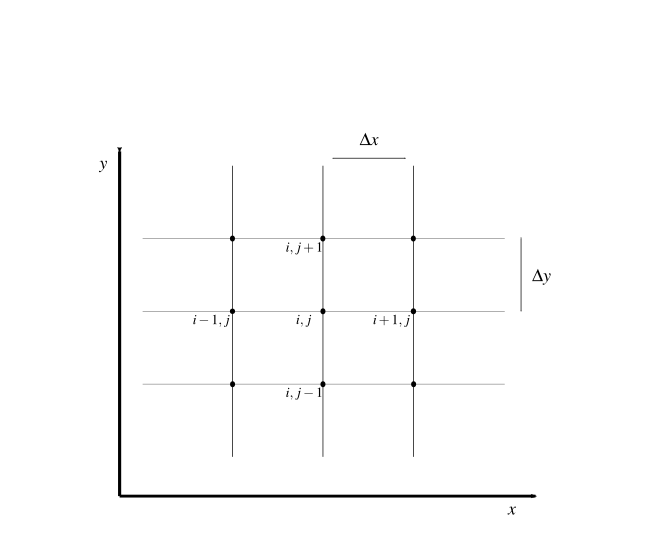
\includegraphics[width=95mm]{./Imagenes/malla-DF1}
        \caption[Discretización por Diferencias Finitas]{Discretización espacial (malla) por el método de diferencias finitas \cite{anderson-yotros}}
        \label{malla-DF1}
    \end{figure}

    \paragraph*{}
    Todos los términos de la serie truncados se agrupan en un sólo término
    conocido como error de truncamiento y es representado por la simbología
    $O()$. Volviendo a la ecuación (\ref{taylor-forward}) y resolviendo para
    $\left( \pdv{f}{x} \right)_{i,j}$ tenemos:

    \begin{equation}
    \left( \pdv{f}{x} \right)_{i,j} = \frac{f_{i+1, j} - f_{i,j}}{\Delta x} - \left( \pdv[2]{f}{x} \right)_{i,j} \frac{\Delta x}{2} - \left( \pdv[3]{f}{x} \right)_{i,j} \frac{(\Delta x)^2}{6} - \dotsb
    \end{equation}
    o bien:
    \begin{equation*}
    \left( \pdv{f}{x} \right)_{i,j} = \frac{f_{i+1, j} - f_{i,j}}{\Delta x} + O(\Delta x)^2
    \end{equation*}
    que para simplificar, queda:\\
    \begin{equation}
    \left( \pdv{f}{x} \right)_{i,j} = \frac{f_{i+1, j} - f_{i,j}}{\Delta x}
    \label{forward-x1}
    \end{equation}

    \paragraph*{}
    El símbolo $O(\Delta x)$ representa el error de truncamiento de la serie de
    expansión, y para este caso particular se dice que tiene una precisión de
    primer orden, ya que se están despreciando los términos de orden superior.

    \paragraph*{}
    La ecuación \ref{forward-x1} se le conoce como una aproximación tipo
    ``forward'' de primer orden y representa el valor aproximado del valor de la
    derivada parcial $\left( \pdv{f}{x}\right)_{i,j}$ calculada mediante la
    relación lineal del punto $(i,j)$ con el punto $(i+1,j)$. (Figura \ref{fig:grafica-forward})

    \begin{figure}[htbp!]
        \centering
        \subfigure[Aproximación forward]{\label{fig:grafica-forward}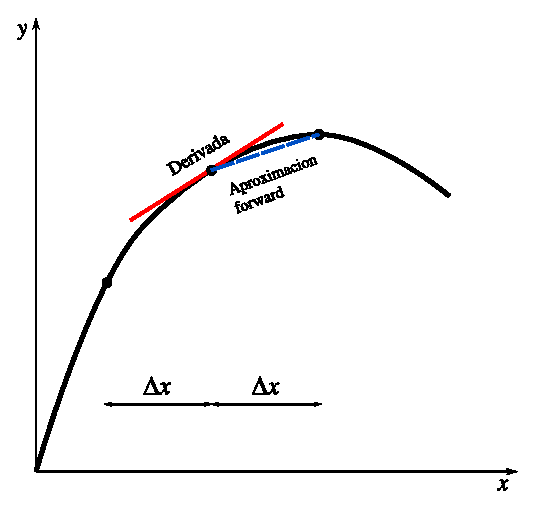
\includegraphics[width=65mm]{./Imagenes/grafica-forward}}
        \subfigure[Aproximación backward]{\label{fig:grafica-backward}\includegraphics[width=65mm]{./Imagenes/grafica-backward}}
        \subfigure[Aproximación central]{\label{fig:grafica-central} 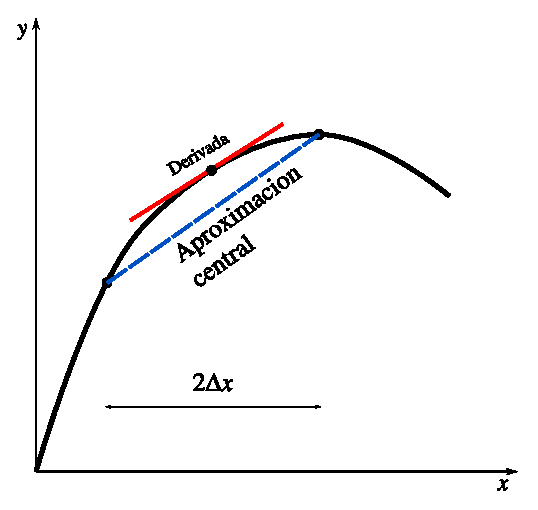
\includegraphics[width=65mm]{./Imagenes/grafica-central}}
        \caption[Aproximaciones por Diferencias Finitas]{Esquemas de las aproximaciones por el método de diferencias finitas.\cite{chapra}}
    \end{figure}

\paragraph*{}
    Para obtener una aproximación tipo ``backward'' se debe generar una serie de Taylor para el punto $(i-1, j)$ expandiendo a partir del punto $(i, j)$
    \begin{equation}
    f_{i-1, j} = f_{i,j} + \left( \pdv{f}{x}\right)_{i,j} \Delta x + \left( \pdv[2]{f}{x} \right)_{i,j} \frac{(-\Delta x)^2 }{2\,!}  + \left( \pdv[3]{f}{x} \right)_{i,j} \frac{(-\Delta x)^3}{3\,!} + \dotsb + \left( \pdv[n]{f}{x} \right)_{i,j} \frac{(-\Delta x)^n}{n\,!}
    \label{taylor-backward}
    \end{equation}
\paragraph{}
    Una vez generada la serie, se sigue el mismo procedimiento empleado en la
    derivación de la aproximación ``forward'' para obtener:
    \begin{equation}
    \left( \pdv{f}{x} \right)_{i,j} = \frac{f_{i,j} - f_{i-1,j}}{\Delta x}
    \label{backward-x1}
    \end{equation}
    \\que es la ecuación de una aproximación ``backward''. (Figura \ref{fig:grafica-backward})

    \paragraph*{}
    Para diferentes aplicaciones de DFC, no basta con tener aproximaciones con
    precisión de primer orden, por lo cual se opta por generar una ecuación que
    tenga una precisión de segundo orden, a esta se le conoce como
    ``aproximación central de segundo orden''. La deducción de ésta, parte de la
    resta de la ecuación \ref{taylor-forward} y la ecuación \ref{taylor-backward},
    que da como resultado:
    \begin{equation}
    f_{i+1,j} - f_{i-1, j} = 2 \left( \pdv{f}{x} \right)_{i,j} \Delta x + 2 \left( \pdv[3]{f}{x} \right)_{i,j} \frac{(\Delta x)^3}{3 \,!} + \dotsb + 2 \left( \pdv[n]{f}{x} \right)_{i,j} \frac{(\Delta x)^n}{n\,!}
    \end{equation}
    que se puede simplificar a:\\
    \begin{equation}
    \left( \pdv{f}{x} \right)_{i,j} = \frac{f_{i+1,j} - f_{i-1,j}}{2 \Delta x}
    \label{central-x1}
    \end{equation}
    se observa en la ecuación \ref{central-x1} que para obtener un coeficiente
    en el punto $(i,j)$ se está utilizando información proveniente de los nodos
    $(i-1, j)$ e $(i+1, j)$, adyacentes a dicho punto. (Figura \ref{fig:grafica-central})

    \paragraph*{}
    Para el análisis de flujos viscosos, además de los coeficientes que sustituyen
    a las derivadas parciales de primer orden se necesitan desarrollar
    aproximaciones para las derivadas parciales de segundo orden, dado que, en
    las ecuaciones que describen el flujo de fluidos viscosos, las ecuaciones de
    Navier-Stokes, los términos de mayor orden son derivadas parciales de
    segundo orden.

    \paragraph*{}
    Si se suman las ecuaciones \ref{taylor-forward} y \ref{taylor-backward}, se
    obtiene un coeficiente para $\pdv[2]{f}{x}$, como se muestra a continuación:
    \begin{equation*}
    f_{i+1,j} + f_{i-1, j} = 2 f_{i,j} + \left( \pdv[2]{f}{x} \right)_{i,j} \frac{(\Delta x) ^2}{2\,!} + \left( \pdv[4]{f}{x} \right)_{i,j} \frac{(\Delta x)^4}{4\,!} + \dotsb + \left( \pdv[n]{f}{x} \right)_{i,j} \frac{(\Delta x)^n}{n\,!}
    \end{equation*}
    despejando la segunda derivada parcial y despreciando el error de truncamiento:
    \begin{equation}
    \left( \pdv[2]{f}{x} \right) = \frac{f_{i+1,j} - 2f_{i,j} + f_{i-1,j}}{(\Delta x)^2}
    \label{central-x2}
    \end{equation}
    a la ecuación \ref{central-x2} se le conoce como aproximación central para
    la derivada de segundo orden.

    \paragraph*{}
    Ahora se desea obtener una aproximación por diferencias finitas para una
    derivada parcial mixta, llámese $\pdv{f}{x}{y}$, donde $f$ es una función
    dependiente de la posición de la partícula de fluido a lo largo de dos ejes,
    $x$ y $y$. Dado que:
    \begin{equation}
    \left( \pdv{f}{x}{y} \right) = \pdv{y} \left( \pdv{f}{x} \right)
    \end{equation}
    podemos desarrollar una aproximacion por diferencias ``central'' de la
    derivada parcial de $y$ en función de $x$, es decir:
    \begin{equation}
    \left( \pdv{f}{x}{y} \right)_{i,j} = \frac{\left( \pdv{f}{y} \right)_{i+1, j} - \left( \pdv{f}{y} \right)_{i-1,j}}{2 \Delta x}
    \end{equation}
    y desarrollando una diferencia central para la derivada parcial de $f$ con
    respecto a $y$ tenemos:
    \begin{equation}
    \left( \pdv{f}{x}{y} \right)_{i,j} = \frac{1}{2 \Delta x} \left[ \frac{f_{i+1, j+1} - f_{i+1, j-1}}{2 \Delta y} - \frac{f_{i-1, j+1} - f_{i-1, j-1}}{2 \Delta y} \right]
    \end{equation}
    \begin{equation}
    \left( \pdv{f}{x}{y} \right)_{i,j} = \frac{1}{4 \Delta x \Delta y} \left( f_{i+1, j+1} + f_{i-1, j-1} - f_{i+1, j-1} - f_{i-1, j+1} \right)
    \end{equation}

    \paragraph*{}
    La misma metodología se aplica para obtener las aproximacinoes por el método
    de diferencia finitas de una función respecto a un eje cualquiera, llámese
    eje $y$, $\xi$ o $\eta$.

    \paragraph*{}
    La mayor ventaja que presenta el método de diferencias finitas es su
    simplicidad de implementación, aunque presenta una limitante, el método
    únicamente es aplicable a mallas estructuradas, además de tampoco poderse
    aplicar a cuerpos de geometría curvilíneas, por lo que es necesario hcer una
    transformación de la malla, de un dominio físico a un dominio lógico, como
    se analiza en el capítulo \ref{chap:mallas}.

    \paragraph*{}
    Es este último punto, la piedra angular en la importancia del desarrollo de
    métodos de generación de mallas, ya que se busca trabajar con mallas en las
    cuales, en sus sistema de coordenadas computacional, pueda ser aplciado el
    método de diferencias finitas para la solución de problemas.
    %
    %
    %
    %
    %

    %
    %
    %
    %
    %
    \chapter{Mallas}
    \label{chap:mallas}
    \paragraph*{}
    Las mallas proveen soporte matemático para llevar a cabo una solución
    numérica de las ecuaciones que gobiernan el campo de análisis como medio
    continuo. La solución numérica se obtiene superponiendo la malla sobre el
    medio continuo, discretizando las ecuaciones respecto a la malla y por
    último, aplicando un algoritmo numérico de solución a la discretización de
    las ecuaciones. Este proceso resulta ser una evaluación de la solución en
    los nodos de la malla.
    \paragraph*{}
    La mecánica de fluidos trabaja con ecuaciones no lineales, las cuales
    describen los flujos de fluidos, dichas ecuaciones en la mayoría de los
    casos prácticos de análisis no pueden ser resueltas de una manera analítica,
    por lo que se ha optado por la solución de dichas ecuaciones mediante
    métodos de aproximaciones entre los cuales encontramos los métodos de
    expansión y perturbación, método de diferencias finitas, método de volúmenes
    finitos e incluso el método de elementos finitos. En general los de mayor
    aplicación práctica son los tres últimos, pero para poder usarlos es
    necesario discretizar el campo de análisis mediante el uso de una malla.\cite{thompsonhandbook}
    \paragraph*{}
    La utilización del método de diferencias finitas es directa si el problema
    se puede expresar en un sistema de coordenadas cartesianas, aunque el mismo
    puede aplicarse a sistemas de coordenadas polares, cilindricas o esféricas,
    dando como resultado una malla rectangular estructurada, con espaciamiento
    uniforme entre los nodos en la dirección de los ejes del sistema. La mayoría
    de casos prácticos de interés en la DFC, tratan con geometrías complejas,
    lo que hace que sea muy dificil, si no imposible, generar una malla en
    alguno de los sitemas de cordenadas antes mencionados, que ajuste en su
    frontera interna de manera exacta a la forma de la geometría a analizar.
    Esto presenta una limitante que se debe atender, se debe llevar a cabo una
    transofrmación de sistemas de coordenadas, llevando el dominio físico del
    problema a un dominio computacional. (Figura \ref{fig:dominios}) El dominio
    computacional es una abstración matemática, mientras que el dominio físico
    es el dominio continuo para el cual se desea una solución numérica.
    \begin{figure}[htbp!]
        \centering
        \includegraphics[width=170mm]{./Imagenes/dominios}
        \caption[Dominios lógico y físico]{Dominios lógico (izquierda) y físico (derecha). \cite{numerical-grid}}
        \label{fig:dominios}
    \end{figure}
    \paragraph*{}
        Una malla es un conjunto de puntos destribuidos a lo largo de un campo
        dentro del cuál se llevaran a cabo los cálculos para obtener la solución
        de ecuaciones diferenciales parciales. Existen dos tipos principales de
        mallas: estructuradas y no estructuradas. (Figura \ref{fig:malla-estructurada-noestructurada})
        Las mallas estructuradas se forman mediante la intersección de
        coordenadas curvilíneas, formando celdas cuadriláteras en dos
        dimensiones, o hexahedros en tres dimensiones. En contraste, las mallas
        no estructuradas no tienen relación alguna con las direcciones
        coordenadas del sistema, éstas consisten generalmente de triángulos y
        tetahédros en dos y tres dimendiones respectivamente, aunque en realidad
        se puede hacer uso de calquier forma geométrica. Para este trabajo se
        considerará el desarrollo  de  mallas estructuradas principalmente, que
        en principio tendrán una forma curvilinea ajustada a la forma del perfil
        alar con el que se esté trabajando como frontera interna del dominio.
    \begin{figure}[htbp!]
        \centering
        \subfigure[Malla Estructurada]{\label{fig:malla-estructurada}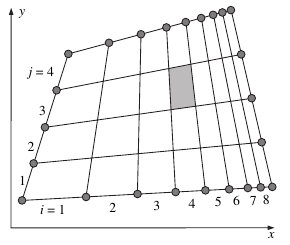
\includegraphics[width=50mm]{./Imagenes/malla-estructurada}} \hspace{20mm} %marca separación entre subfiguras
        \subfigure[Malla no Estructurada]{\label{fig:malla-no-estructurada}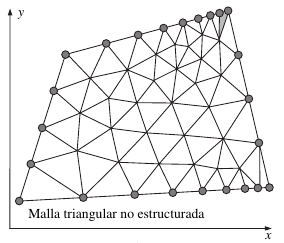
\includegraphics[width=50mm]{./Imagenes/malla-no-estructurada}}
        \caption[Mallas estructuradas y no estructuradas]{Mallas estructuradas
        y no estructuradas.\cite{cengel}}
        \label{fig:malla-estructurada-noestructurada}
    \end{figure}

    \paragraph*{}
        La malla debe de generarse bajos ciertas restricciones las cuales suelen
        ser difíciles de satisfacer por completo. En la actualidad el tiempo que
        toma generar una malla llega a ser mayor en órdenes de magnitud que el
        tiempo requerido para la construcción y análisis de la solución del
        flujo sobre la malla. En especial ahora que hay mayor disponibilidad de
        software para la solución de flujos.\cite{thompsonhandbook}

\section{Tipos de Mallas Estructuradas}
    \paragraph*{}
        Existen tres tipos base de mallas conocidos como mallas C, H u O
        respectivamente. El nombre que dichos tipos de mallado reciben se debe
        a que su estructura asemeja a dichas letras (en mayúsculas) desde una
        vista de planta.

        \begin{figure}[htbp!]
            \centering
            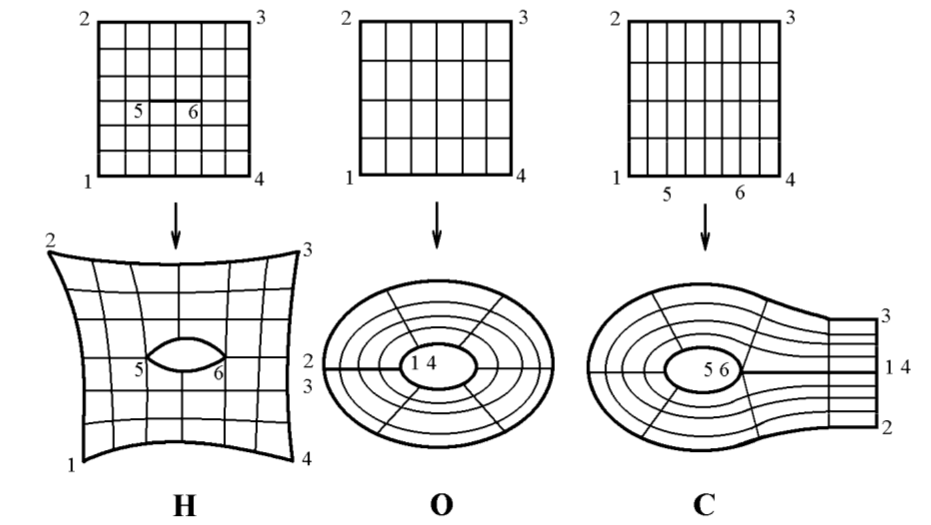
\includegraphics[width=170mm]{./Imagenes/tipos-de-malla}
            \captionsetup{justification=centering, margin=2cm}
            \caption[Tipología de mallas]{Tipología de malla y sus respectivos espacios computacionales. H(izquierda), O(centro), C(derecha).\cite{vladimir-grid}}
            \label{fig:tipos-de-malla}
        \end{figure}

    \subsection{Mallas tipo C}
    \paragraph*{}
        Las mallas tipos C están compuestas por una sección semicircular y otra
        rectangular en la frontera exterior, mientras que la frontera interior
        es de la misma forma del objeto que se analiza.
    \paragraph*{}
        Suelen utilizarse para el análisis de flujos alrededor de perfiles
        alares, pues ofrecen como principal ventaja un buen análisis del flujo
        en la zona de deflexión de la estela, en especial si se compara contra
        las mallas tipo O.\cite{best-practices-grid-generation}
    \paragraph{}
        La transformación de esta malla de un espacio físico a un espacio
        computacional da como resultado una malla conformada por rectangulos.
        Durante la transformación se debe identificar un segmento, tambien
        conocido como corte, ya que este proceso implica conceptualemte, una
        separación en dicho corte, para posteriormente deformar el espacio
        físico llevándolo así a convertirse en una malla estructurada uniforme.
        En la figura \ref{fig:malla-c} se observa que en el dominio físico, el
        segmento $(ab)$ representa la sección del mallado donde se realiza el
        corte y que tambien se le llama $(a'b')$, y que en el dominio
        computacional este segmento representa dos segmentos diferentes.
            \begin{figure}[htbp!]
                \centering
                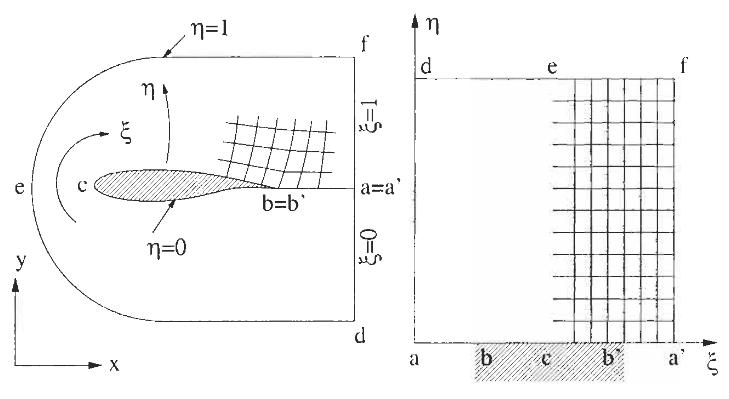
\includegraphics[width=155mm]{./Imagenes/malla-c}
                \captionsetup{justification=centering, margin=2cm}
                \caption[Malla tipo C]{Malla tipo C y su transformación del espacio físico (izquierda) al espacio lógico (derecha). \cite{blazek}}
                \label{fig:malla-c}
            \end{figure}
    \subsection{Mallas tipo O}
    \paragraph*{}
        Este tipo de mallas son principalmente de sección circular, de ahí su
        nombre. Suelen ser utilizadas para el análisis del flujo alrededor de
        algunos componentes de aeronaves, como puede ser el fuselaje o las
        góndolas, entre otros.\cite{vladimir-grid} Tambien pueden llegar a
        utilizarse en el análisis de perfiles alares, pero presentan la
        dificultad de ofrecer una baja calidad de mallado en el borde de salida.\cite{blazek}\cite{best-practices-grid-generation}
    \paragraph*{}
        En este caso, al igual que sucede con las mallas tipo C, el resultado en
        el dominio lógico es un cuadrado.El proceso de transformación de este
        tipo de malla se puede conceptualizar como el desdoble del espacio
        físico a partir de un corte, en la figura \ref{fig:malla-o} se
        representa como $(ac)$ o como $(a'c')$, para después deformarlo hasta
        alcanzar la forma cuadrada esperada.
            \begin{figure}[htbp!]
                \centering
                    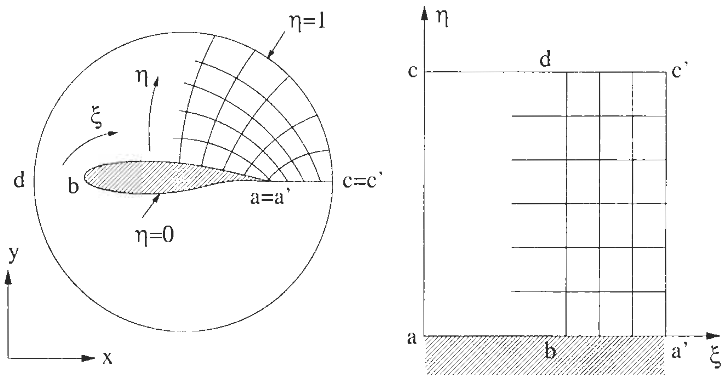
\includegraphics[width=170mm]{./Imagenes/malla-o}
                    \captionsetup{justification=centering, margin=2cm}
                    \caption[Malla tipo O]{Malla tipo O y su transformación del
                    espacio físico (izquierda) al espacio lógico (derecha).\cite{blazek}}
                \label{fig:malla-o}
            \end{figure}
    \subsection{Mallas tipo H}
    \paragraph*{}
        Este tipo de mallas son utilizadas principalmente en los análisis de
        turbomaquinaria, específicamente en la zona de los alabes.\cite{blazek}\cite{best-practices-grid-generation}
        Tambien suelen utilizarse en el análisis de alas de aeronaves.\cite{vladimir-grid}
    \paragraph*{}
        La transformación en este tipo de malla, tambien da como resultado un
        dominio computacional cuadrado, que puede tener o no un corte al
        interior el cual corresponde a la frontera interior del dominio físico.
        (Figura\ref*{fig:tipos-de-malla} (H)) La frontera externa del dominio
        computacional corresponde a la frontera externa del dominio físico.

    \paragraph*{}
        La figura\ref{fig:malla-h} muestra el uso de una malla tipo H para el
        análisis del flujo a través de los álabes de una turbina, y su
        transformación del dominio físico al computacional. En este caso no
        existe un cuerpo en el centro del mallado, por lo que no hay corte
        alguno en el dominio lógico.
            \begin{figure}[htbp!]
                \centering
                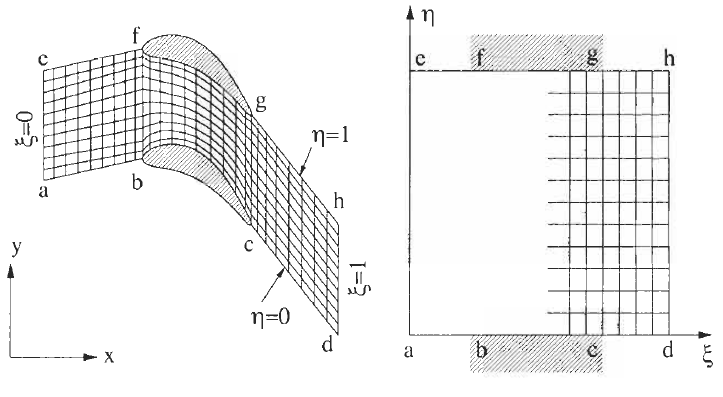
\includegraphics[width=170mm]{./Imagenes/malla-h}
                \captionsetup{justification=centering, margin=2cm}
                \caption[Malla tipo O]{Malla tipo H y su transformación del espacio físico (izquierda) al espacio lógico (derecha). \cite{blazek}}
            \label{fig:malla-h}
            \end{figure}

    \paragraph*{}
        En el caso de que se quiera ocupar una malla H con un cuerpo a analizar
        en el interior del dominio, como el caso representado en la figura\ref*{fig:tipos-de-malla} (H)
        se puede realizar un mallado uniforme, quizás mediante un método de
        interpolación algeráica, sobre el dominio físico quedando así
        coincidente con el dominio computacional. Los puntos 5 y 6 requieren de
        un trato especial al momento de llevar a cabo la solución, un ejemplo de
        esto puede ser que todos los puntos del mallado que caen dentro del
        objeto de análisis no sean utilizados durante la solución.

    \section{Mallas Adaptativas}
    \paragraph*{}
        A pesar de que existen varios modelos algebráicos y diferenciales para
        la generación de mallas, aún hay problemas para los cuales estos métodos
        no generen una malla adecuada, ya sea que la malla se aleje mucho de la
        ortogonalidad en ciertos puntos, que esté coprimida, e incluso no se
        llegue a la convergencia. Desde la década de 1960, época en la que la
        generación de mallas comienza a ser estudiada con mayor seriedad, se han
        analizado enfoques variables para solucionar los problemas presentados
        en los enfoques diferenciales.

    \section{Consideraciones preliminares para la generación de mallas}
    \paragraph*{}
        La densidad de la malla es el primer aspecto que se debe considerar, se
        debe generar una malla solo sufcientemente densa para que la
        aproximación numérica sea precisa, sin embargo, se debe tener cuidado en
        no hacer la malla demasiado densa, tanto que resulte impractico llevar a
        cabo un análisis y llegar a una eventual solución.
    \paragraph{}
        Otro importante aspecto a tener en cuenta durante este proceso, es la
        eficiencia computacional. Por un lado el uso de memoria podría ser tan
        grande que resulte impractico llevar a cabo este proceso, por lo que una
        organización adecuada de la información es de vital importancia. Por
        otro lado, la generación de mallas debe llevarse a cabo mediante la
        implementación de códigos lo menos complejos posible.

    \section{Técnicas de generación del mallado}
    \paragraph*{}
        La generación de mallas \textit{per se}, es un proceso libre durante su
        desarrollo, es decir, no se lleva a cabo mediante alguna fórmula o
        procedimiento estricto, por lo tanto, cualquier desarrollo se puede
        considerar apto para este propósito siempre y cuando dé como resultado
        una mallado adecuado para el análisis que se pretende realizar. Sin
        embargo, si hay ciertas consideraciones a tomar en cuenta, tales como la
        capacidad de manejar problemas con múltiples variables, las cuales
        podrían variar en varios órdenes de magnitud. Del mismo modo, se debe
        considerar la posibilidad de presentar factores de compresión en ciertas
        áreas de la malla, en contraste con una malla uniforme.

    \paragraph*{}
        Podemos señalar principalmente dos tipos de técnicas para la generación
        de mallado, de entre el amplio número de técnicas existentes al día de
        hoy, las cuales son:
        \begin{itemize}
            \item Métodos algebráicos: es de todos, el método más sencillo de
                implementar, una de sus ventajas es la rapidez con la que se
                genera la malla. Se utiliza un método de interpolación para
                determinar los nodos del mallado, partiendo de las coordenadas
                de la frontera externa e interna. Y se realiza la transformación
                del dominio físico al lógico mediante una ecuación algebráica.
            \item Metódos mediante  ecuaciones diferenciales parciales (EDP): se
                resuelve una EDP para obtener la distribución de los nodos,
                la resolución de las mismas se lleva a cabo mediante
                aproximaciones por el método de diferencias finitas. La
                distribución de la malla puede ser uniforme o concentrada
                dependiendo del tipo de ecuación que se resuelva.
        \end{itemize}

\section{Generación de mallas mediante métodos algebráicos}
    \paragraph*{}
        Como ya se mencionó previamente, los métodos más eficientes para la
        generación de mallas son los métodos algebráicos. Éstos métodos basados
        en interpolación son de gran utilidad en la industria, debido a su
        sencilla implementación, además de la capacidad de control sobre la
        densidad de la malla respecto a un nodo dentro del dominio. Un aspecto
        en contra de la generación de mallas mediante estos métodos es que no
        tienen la capacidad de suavizar las curvas, si no que tienden a mantener
        la forma de las fronteras, por lo que si se llegara a presentar algún
        tipo de discontinuidad en la frontera interna (superficie de análisis),
        esta seguiría presente los nodos internos de la malla. Es por esto que
        estos métodos son utilizados de manera general, como una primera
        aproximación, la cual sirve como condición inicial en la generación de
        mallas mediante la solución de sistemas de ecuaciones diferenciales
        parciales.\cite{farrashkhalvat}
    \paragraph*{}
        La idea fundamental sobre la cual se desarrollan todos los métodos
        algebráicos es el uso de funciones de interpolación matemática para
        interpolar entre algunos puntos conocidos o previamente asignados
        (fronteras) para así obtener la distribución de puntos que se ubican
        entre los ya mencionados. El método de interpolación puede variar
        dependiendo del método algebráico que se esté empleando, pero la idea
        base permanece.\cite{siladicParabolic}
    \paragraph*{}
        Los métodos algebráicos relacionan un dominio computacional, descrito
        por un cuadrado en 2D y un cubo en 3D, con un dominio físico de
        geometría arbitraria.

    \subsection{Interpolación unidireccional}
    \paragraph*{}
        La interpolación unidireccional se lleva a cabo interpolando una línea
        a la vez, en una dirección del espacio computacional, ya sea $\xi$ o
        $\eta$. Es decir, para interpolar en la dirrección $\xi$ (desarrollo que
        se presenta en este trabajo), se deben seleccionar puntos en las
        frontera tanto interna como externa, que correspondan a la misma línea
        $\eta = constante$ y a lo largo de la cual se hará la interpolación,
        haciendo la variación en la coordenada $\xi$, interpolando así, línea
        por línea hasta terminarse de generar la malla. El mismo procedimiento
        se puede llevar a cabo interpolando en la dirección de $\eta$.
    \subsubsection{Interpolación Polinomial}\label{Lagrange}
    \paragraph*{}
        En este método se ocupa el polinomio de Lagrange como ecuación de
        interpolación para generar la malla.
        \begin{align}
            L_{i}(x) = \frac{(x - x_{0})(x - x_{1}) \dotsb (x - x_{i-1}) (x - x_{i+1}) \dotsb (x - x_{n})}{(x_{i} - x_{0} )(x_{i} - x_{1}) \dotsb (x_{i} - x_{i-1}) (x_{i} - x_{i+1}) \dotsb (x_{i} - x_{n}) } && i = 0, 1, \dotsc , n
        \end{align}
        \\El polinomio resultante será de grado $n$, donde el numerador omite el término $(x - x_{i})$

    \paragraph*{}
        El caso más sencillo con el que se puede trabajar el polinomio de
        Lagrange es generando un polinomio de grado 1, que resulta ser una línea
        recta que pasa a través de dos puntos $(x_{0} , y_{0})$ y $(x_{1}, y_{1})$,
        los cuales pertenecen a la frontera interna y externa respectivamente.
        Para este caso, se tienen los siguientes términos:
        \begin{align*}
            L_{0} = \frac{ ( x - x_{1} ) }{ (x_{0} - x_{1} ) } && L_{1} = \frac{ ( x - x_{0} ) }{ (x_{1} - x_{0} ) }
        \end{align*}
        dando como resultado la ecuación que describe a una recta
        \begin{equation}
            y = y_{0} \frac{ ( x - x_{1} ) }{ ( x_{0} - x_{1} ) }  + y_{1} \frac{ (x - x_{0})  }{( x_{1} - x_{0} )} = y_{0} (1 - \xi) + y_{1}\xi
        \end{equation}
        de donde se sabe que
        \begin{equation}
            \xi = \frac{x - x_{0}}{x_{1} - x_{0}}
            \label{xi}
        \end{equation}
        y se observa que $\xi = 0, 1$ cuando $x = x_{0}, x_{1}$ respectivamente.
    \paragraph*{}
        Despejando $x$ de la ecuación\ref{xi} se obtiene:
        \begin{equation}
            x = (x_{1} - x_{0})\xi - x_{0} = x_{0}(1 - \xi) + x_{1}\xi
        \end{equation}
        por lo que la ecuación constitutiva de éste método, para una
        interpolación en dirección del eje $\xi$ del espacio computacional puede
        escribirse de la siguiente manera:
        \begin{equation}
            r(\xi, \eta_{j}) = (1 - \xi_{i}) r(0, \eta_{j}) + \xi_{i}r(1, \eta_{j})
        \end{equation}

    \paragraph*{}
        Se puede hacer uso de la generación de un polinomio de mayor grado, para
        lo cual se deben proporcionar más puntos previamente definidos por los
        cuales tiene que pasar la curva descrita del polinomio. Para generar una
        ecuación de grado $n$ se deben proporcionar como datos de inicio, al
        menos $n+1$, es decir, si se quisiera hacer la interpolación mediante un
        polinomio de grado 2, se debe proporcionar la información de al menos 3
        puntos. Siempre cabe la posibilidad de que los puntos pertenezcan a una
        linea recta, en cuyo caso los términos de mayor orden se verán
        eliminados.
    \paragraph*{}
        Las figuras\ref{fig:malla-inter} y\ref{fig:malla-inter-cerca}
        presentan una malla y su vista de detalle generada mediante este método
        alrededor de un perfil aerodinámico.
        \begin{figure}[htbp!]
            \centering
            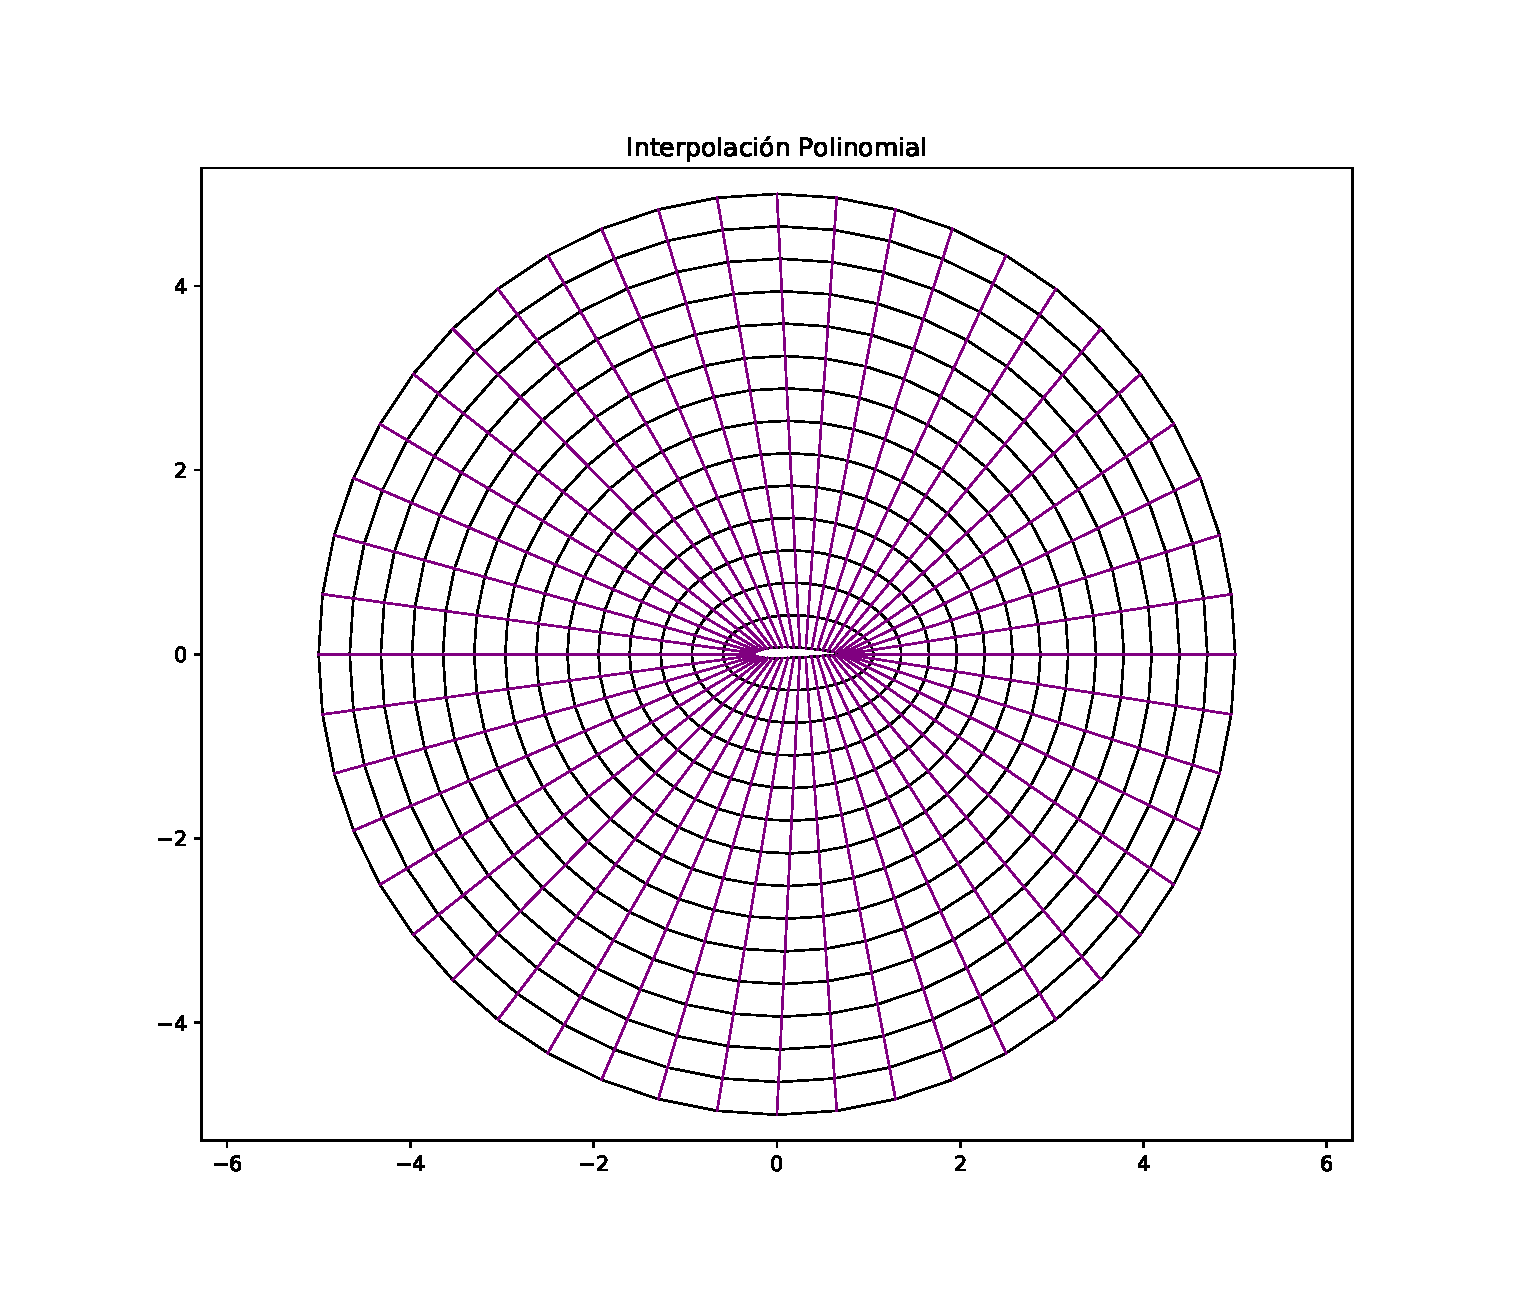
\includegraphics[width=120mm]{./Imagenes/M-inter_pol}
            \captionsetup{justification=centering, margin=2cm}
            \caption[Malla Interpolación Polinomial]{Malla tipo O generada
            mediante el método de interpolación polinomial alrededor de un
            perfil NACA 2412. Densidad de malla $49\times15$}
            \label{fig:malla-inter}
        \end{figure}
        \begin{figure}[htbp!]
            \centering
            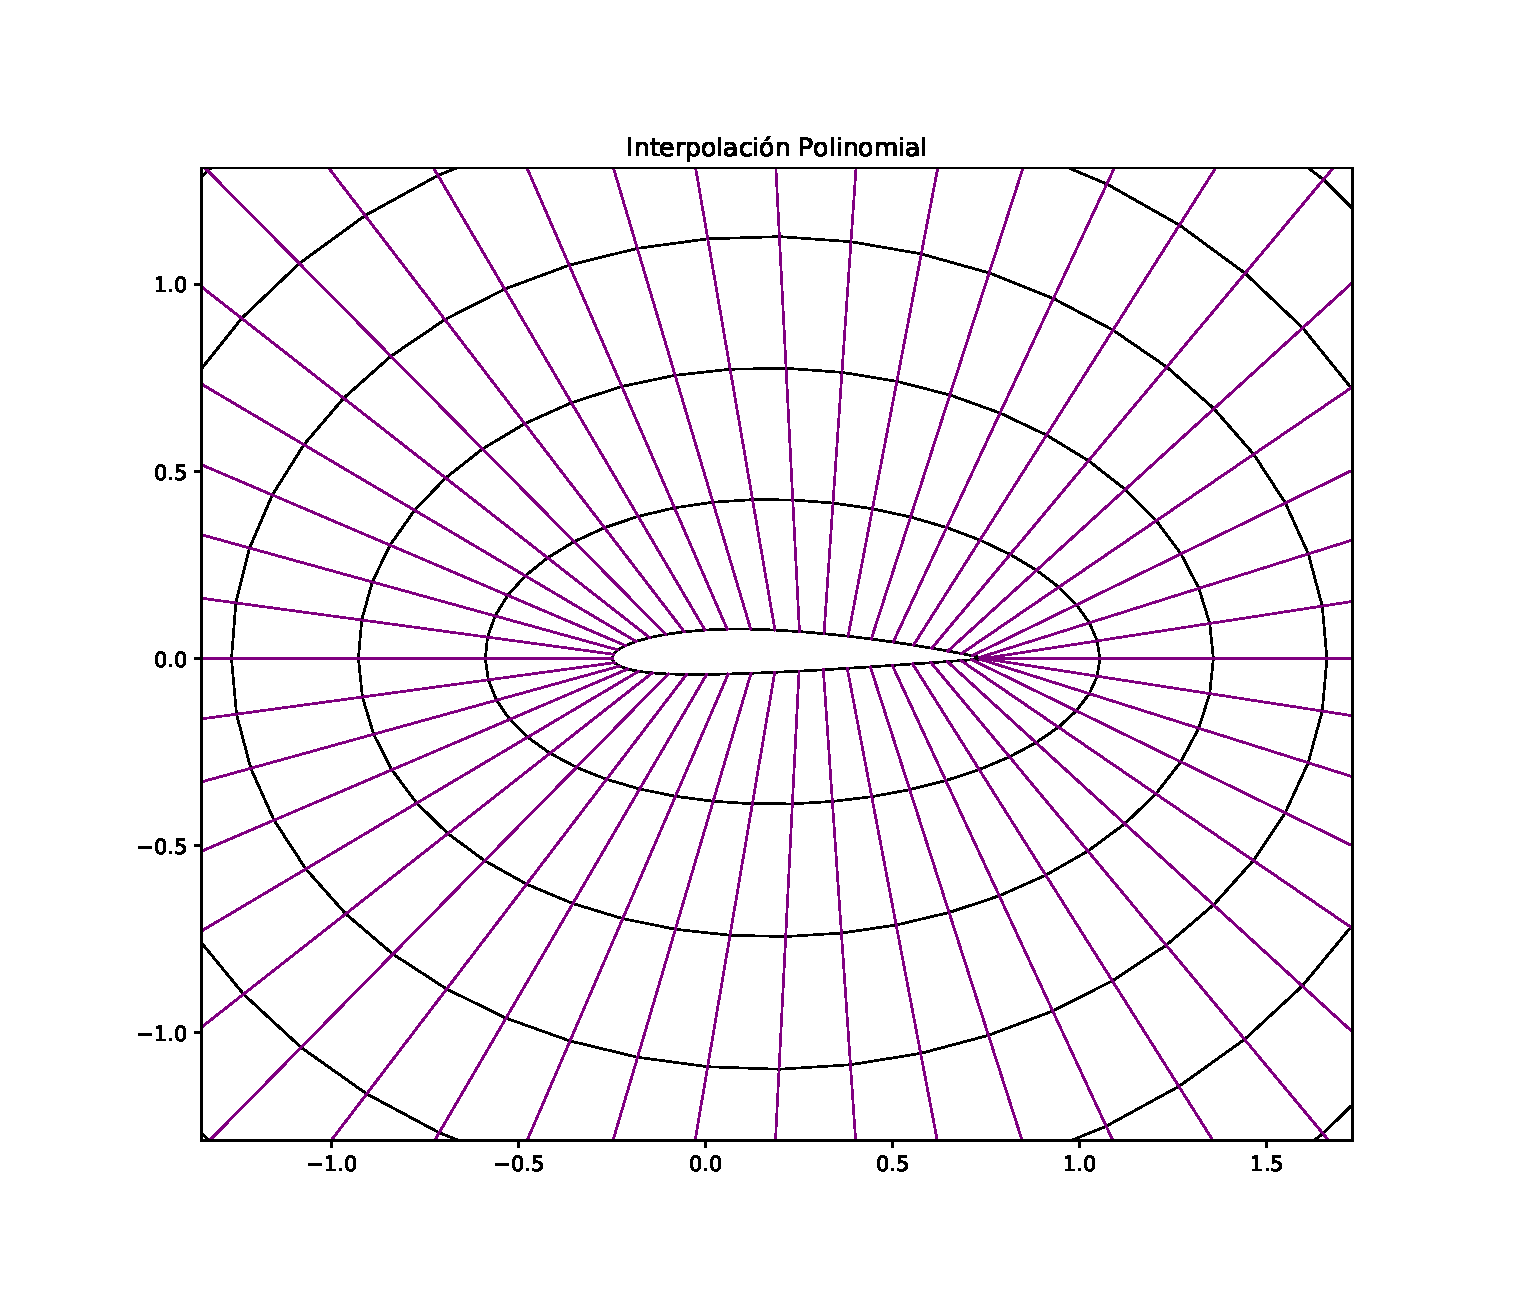
\includegraphics[width=120mm]{./Imagenes/M-inter_pol_cerca}
            \captionsetup{justification=centering, margin=2cm}
            \caption[Malla Interpolación Polinomial Acercamiento]{Vista de
            acercamiento a la malla generada de la figura\ref{fig:malla-inter}}
            \label{fig:malla-inter-cerca}
        \end{figure}

    \subsubsection{Interpolación mediante polinomios de Hermite}
    \paragraph*{}
        La interpolación mediante el polinomio de Lagrange se realiza mediante
        el uso de valores conocidos de ciertos puntos, sin embargo, es posible
        generar una malla partiendo tanto de valores conocidos de una función
        como de los valores de su primer derivada para ciertos puntos dados.
        El polinomio que describe este método se escribe como:
        \begin{equation}
        p(x) = \sum_{i = 0}^{n} y_{i}H_{i}(x) + \sum_{i = 0}^{n}y_{i}\prime \widetilde{H}_{i}(x)
        \end{equation}

    \paragraph*{}
        Los siguientes polinomios definen los polinomios de Hermite $H_{i}(x) \widetilde{H}_{i}(x)$
        en función de polinomios de Lagrange:
        \begin{equation}
            H_{i}(x) = \{  1 - 2L\prime_{i}(x_{i})(x - x_{i})  \} \left[L_{i}\right]^2
        \end{equation}
        \begin{equation}
            \widetilde{H}_{i}(x) = (x - x_{i}) \left[L_{i}\right] ^ 2
        \end{equation}
    \paragraph*{}
        Se suele usar polinomios de Hermite cubicos, para los cuales se requiere
        el uso de polinomios de Lagrange de primer grado, es decir polinomios
        lineales. La ecuación constitutiva de la interpolación en dirección del
        eje $\xi$, por polinomios cúbicos de Hermite queda expresada de la
        siguiente manera:
        \begin{equation}
            r(\xi) = \sum_{i = 0}^{n} r_{i}H_{i}(\xi) + \sum_{i = 0}^{n} r\prime_{i}\widetilde{H}_{i}(\xi)
        \end{equation}
        que a su vez, desarrollando las operaciones matemáticas, se expresa como:
        \begin{align}
            &\begin{aligned}
                r(\xi, \eta_{j}) =& r(0, \eta_{j})(2\xi^3 - 3\xi^2 +1) + r(1, \eta_{j})(3\xi^2 - 2\xi^3) \\ &+ r\prime(0, \eta_{j})(\xi^3 - 2\xi^2 + \xi) + r\prime(1, \eta_{j})(\xi^3 - \xi^2)
            \end{aligned}
        \end{align}

    \subsection{Interpolación multidireccional}
    \paragraph*{}
        La interpolación multidireccional consiste en la obtención de una
        ecuación algebráica que permita la interpolación simultánea en 2 o más
        direcciones. Para este caso (2D), se generan ecuaciones que permitan la
        interpolación simultánea, en el espacio computaciones, en ambas
        direcciones $\xi$ y $\eta$.
    \subsubsection{Interpolación Transfinita - TFI}
    \paragraph*{}
        El método de TFI es un método de interpolación multivariable. Cuando se
        aplica el TFI para la generación de mallas, se restringe la malla para
        que coincida con la fronteras especificadas. Este método consiste en la
        suma de las interpolaciones de una sola variable para cada una de las
        coordenadas computacionales. Existen diversos tipos de interpolación a
        lo largo de una coordena, por lo que existen práctimanete un número
        ilimitado de variantes de TFI creadas a partir de la combinación de
        diversas interpolaciones de una sola variable.\cite{thompsonhandbook}
    \paragraph*{}
        Una de las principales ventajas del método de interpolación transfinita
        es que asegura una concordancia en las fronters en ambas direcciones.
        Su escencia es la de la interpolación en cada una de las coordenadas
        computacionales, formando así los productos tensores de las
        interpolaciones, y finalmente, se lleva a cabo una suma ``booleana''.
        Las interpolaciones unidireccionales son una combinación lineal de datos
        proporcionados por el usuarios del dominio físico para valores dados de
        las coordenadas del dominio lógico.
    \paragraph*{}
        A partir de la existencia de una transformación $r = r(\xi, \eta)$
        ($x = x(\xi, \eta), y = y(\xi, \eta)$ la cual hace un mapeo de un
        cuadrado de dimensiones $0 < \xi < 1, 0 < \eta < 1$ en el dominio
        computacional, con la región del dominio físico, delimitada por una
        frontera externa y una interna, que se pretende analizar.
        De igual modo, se puede escribir otra transformación $P_{\xi}$,
        la cual recibe el nombre de proyector, la cual relaciona puntos en el
        espacio lógico con puntos en el espacio físico, definida como:
        \begin{equation}
            P_{\xi}(\xi, \eta) = (1 - \xi)r(0, \eta) + \xi r(1, \eta)
        \end{equation}
    \paragraph*{}
        Como ya se explicó en la sección \ref{Lagrange}, esta tranformación hace
        una transformación con la cual las fronteras en la dirección de $\xi$
        son mapeadas, mientras que las fronteras en dirección de $\eta$ son
        reemplazadas por lineas rectas. De manera análoga se puede definir el
        proyector:
        \begin{equation}
            P_{\eta}(\xi, \eta) = (1 - \eta)r(\xi, 0) + \eta r(\xi, 1)
        \end{equation}
        con el cual se preservan las fronteras en dirección $\eta$ y se
        reemplazan las fronteras en $\xi$ por líneas rectas.
        \begin{figure}[htbp!]
            \centering
            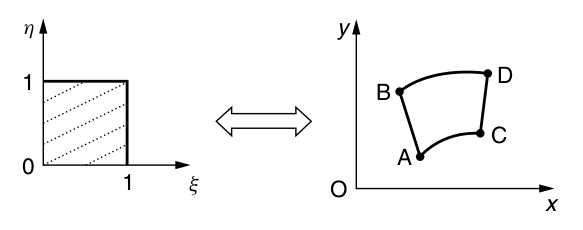
\includegraphics[width=120mm]{./Imagenes/mapeo_eta}
            \caption[Transformación de malla por $P_{\eta}$]{Transormación de
            una malla a través del proyector $P_{\eta}$ \cite{farrashkhalvat}}
            \label{fig:mapeo_eta}
        \end{figure}
    \paragraph*{}
        La figura \ref{fig:mapeo_eta} representa gráficamente la transformación
        de la malla del dominio lógico al dominio computacional mediante la
        aplicación del proyector $P_{\eta}$. Se observa como las fronteras
        conformadas por los segmentos $AC$ y $BD$ se conservan durante las
        transformación, mientras que las fronteras $AB$ y $CD$ son reemplazadas
        por líneas rectas.
    \paragraph*{}
        A partir de estas ecuaciones, se uede definir un mapeo compuesto
        $P_{\xi}P_{\eta}$, de tal manera que:
        \begin{align}
            \begin{aligned}
                P_{\xi}(P_{\eta}(\xi, \eta)) &= P_{\xi} ((1 - \eta)r(\xi, 0) + \eta r(\xi, 1)) \\
                &= (1 - \xi) \left[ (1 - \eta)r(0, 0) + \eta r(0, 1) \right] + \xi \left[ (1 - \eta)r(1, 0) + \eta r(1,1) \right]\\
                &= (1 - \xi)(1 - \eta)r(0, 0) + (1-\xi)\eta r(0, 1) + \xi(1 - \eta)r(1, 0) + \xi\eta r(1, 1)
            \end{aligned}
        \end{align}
    \paragraph*{}
        Con esta transformación compuesta, se logra preservar los 4 vértices en
        los que se interseccionan las fronteras, sin embargo, las cuatro
        fronteras son reemplazadas por líneas rectas. Es decir, las líneas
        $\xi = constante$ y $\eta = constante$ en el dominio computacional son
        transformadas como líneas rectas en el dominio físico, como se muestra
        en la figura\ref{fig:mapeo_xieta}.
        \begin{figure}[htbp!]
            \centering
            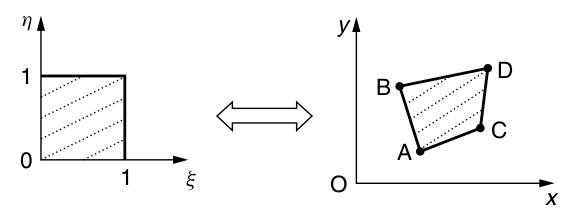
\includegraphics[width=120mm]{./Imagenes/mapeo_xieta}
            \caption[Transformación de malla por $P_{\xi}P_{\eta}$]{Transormación
            de una malla a través del proyector compuesto
            $P_{\xi}P_{\eta}$\cite{farrashkhalvat}}
            \label{fig:mapeo_xieta}
        \end{figure}

    \paragraph*{}
        Si consideramos los diferentes mapeos de un lado, bajo cualquiera de los
        proyectores previamente desarrollados, por ejemplo el lado $\eta = 0$,
        bajo el proyector $P_{\xi}$ es mapeado con una línea recta $AC$, si por
        otro lado se lleva a cabo la transformación medainte el proyector
        $P_{\eta}$ el mapeo resultante es uno a uno, es decir que la recta
        $\eta = 0$ se mapea con la curva de la frontera $AC$. Por último
        transformando con el proyector compuesto $P_{\xi}P_{\eta}$ tambien se
        hace un mapeo con la línea recta $AC$.
    \paragraph*{}
        Desarrollando la misma lógica y consideraciones a las 4 fronteras de la
        frontera, se concluye que el mapeo compuesto $(P_{\xi} + P_{\eta} - P_{\xi}P_{\eta})$
        lleva a cabo una transformación con un mapeo uno  a uno de las fronteras
        del cuadrado de longitud uitaria (dominio computacional) con la curvas
        de frontera del dominio físico. A este mapeo se le conoce como la suma
        booleana de las transformaciones $P_{\xi}$ y $P_{\eta}$, y se escribe
        $P_{\xi}\oplus P_{\eta}$, por lo tanto:
        \begin{equation}
            P_{\xi}\oplus P_{\eta} = P_{\xi} + P_{\eta} - P_{\xi} P_{\eta}
        \end{equation}
        con lo que la fórmula final queda:
        \begin{align}
            \begin{aligned}
                \left( P_{\xi}\oplus P_{\eta} \right)(\xi, \eta) =& P_{\xi}(\xi, \eta) + P_{\eta}(\xi, \eta) - P_{\xi}P_{\eta}(\xi, \eta) \\
                =& (1 - \xi)r(0, \eta) + \xi r(1, \eta) + (1 - \eta)r(\xi, 0) + \eta r(\xi, 1) \\&- (1-\xi)(1 - \eta)r(0, 0) - (1 - \xi)\eta r(0, 1) - (1- \eta)\xi r(1, 0) \\& - \xi \eta r(1,1)
            \end{aligned}
        \end{align}
    \paragraph*{}
            Esta ecuación es la base del métro de TFI para dos dimensiones. La
            malla se genera tomando valores discretos $\xi_{i}, \eta_{j}$ para
            los ejes $\xi$ y $\eta$.

\section{Generación de mallas mediante EDP}
    \paragraph*{}
        La generación de mallas mediante estos métodos se ha esparcido gracias a
        la versatilidad que poseen y la relativa facilidad con la que pueden ser
        aplicados. La idea sobre la cual se desarrolla el método, es la de
        obtener la solución númerica de una ecuación diferencial parcial, esta
        solución representa las coordenadas de la malla, la cual debe coincidir
        en su frontera interna, con la forma geométrica del cuerpo que se
        pretende analizar.\cite{siladicParabolic}

    \paragraph*{}
        Existen tres esquemas predominantes de generación de mallas mediante la
        solución de sistemas de ecuaciones diferenciales parciales:
        \begin{itemize}
            \item Ecuaciones Elípticas
            \item Ecuaciones Hiperbólicas
            \item Ecuaciones Parabólicas
        \end{itemize}

    \subsubsection{Generación de mallas mediante EDP elípticas}
    \paragraph*{}
        Para la solución de un sistema de EDP elípticas se necesita cumplir la
        condición de tener definidas las condiciones de frontera a lo largo de
        todos los puntos pertenecientes a la misma, es decir, que se tengan
        condiciones de frontera de Dirichlet.
        La solución se obtiene mediante diferentes métodos numéricos iterativos
        entre los que destacan el método de Jacobi, el método de Gauss-Seidel y
        métodos de sobre relajación. Informacion sobre el procedimiento y
        desarrollo de estos métodos está disponible en el apéndice \ref{appIter}.
    \paragraph*{}
        La idea es que se calculen las coordenadas $(\xi, \eta)$ y que la
        solución del sistema de ecuaciones genere las correspondientes
        coordenadas $(x, y)$ del dominio físico, con un mapeo uno a uno, es
        decir, que exista una relación adecuada entre el dominio computacional y
        el lógico.

    \paragraph*{}
        Considerando la ecuación de Laplace:
        \begin{subequations}
            \begin{equation}
                \xi_{xx} + \xi_{yy} = 0
            \end{equation}
            \begin{equation}
                \eta_{xx} + \eta_{yy} = 0
            \end{equation}
            \label{ec-laplace}
        \end{subequations}\\
        donde como ya se ha mencionado, $\xi$ y $\eta$ representan las
        coordenadas del dominio computacional y además, son variables
        dependientes de $x$ y de $y$. Si se quiere trabajar con la forma
        inversa, es decir, que ahora $x$ y $y$ sean variables dependientes de
        $\xi$ y $\eta$, la ecuación  de Laplace se expresa como:
        \begin{subequations}
            \begin{equation}
                \alpha x_{\xi \xi} - 2\beta x_{\xi \eta} + \gamma x_{\eta \eta} = 0
            \end{equation}
            \begin{equation}
                \alpha y_{\xi \xi} - 2\beta y_{\xi \eta} + \gamma y_{\eta \eta} = 0
            \end{equation}
            \label{ec-laplace-invertida}
        \end{subequations}\\

        donde:
        \begin{equation*}
            \alpha = x_{\eta} ^ 2 + y_{\eta}^2
        \end{equation*}
        \begin{equation*}
            \beta = x_{\xi} x_{\eta} + y_{\xi} y_{\eta}
        \end{equation*}
        \begin{equation*}
            \gamma = x_{\xi} ^ 2 + y_{\xi} ^ 2
        \end{equation*}

    \paragraph*{}
        La distribución de los nodos, obtenidos mediante la solución de la
        ecuación de Laplace (ecuación \ref{ec-laplace}), tiende ser uniforme
        debido al efecto suavizante de dicha ecuación. Para poder manipular esta
        distribución, es necesario agregar funciones de forzado a la ecuación
        \ref{ec-laplace}, dando como resultado la ecuación de Poisson:
        \begin{subequations}
            \begin{equation}
                \xi_{xx} + \xi_{yy} = P(\xi, \eta)
            \end{equation}
            \begin{equation}
                \eta_{xx} + \eta_{yy} = Q(\xi, \eta)
            \end{equation}
            \label{ec-poisson}
        \end{subequations}

        y transformando la ecuación, haciendo $x$ y $y$ las variables
        dependientes:
        \begin{subequations}
            \begin{equation}
                \alpha x_{\xi \xi} + \beta x_{\xi \eta} + \gamma x_{\eta \eta} = -I^2 [P(\xi, \eta) x_{\xi} + Q(\xi, \eta) x_{\eta}]
            \end{equation}
            \begin{equation}
                \alpha y_{\xi \xi} + \beta y_{\xi \eta} + \gamma y_{\eta \eta} = -I^2 [P(\xi, \eta) y_{\xi} + Q(\xi, \eta) y_{\eta}]
            \end{equation}
            \label{ec-poisson-invertida}
        \end{subequations}

    \paragraph*{}
        Las funciones $P$ y $Q$ se seleccionan dependiendo de la necesidad
        específica del problema que se analiza. Dichas necesidades pueden ser,
        por ejemplo, el agrupamiento de nodos alrededor de un punto especifico,
        o quizás sea la búsqueda de un sistema ortogonal en la superficie.

    \paragraph*{}
        El uso de las funciones $P$ y $Q$ para manipular la densidad de puntos
        alrededor de ciertas zonas se logra atrayendo las líneas vecinas a una
        línea seleccionada. La misma funciona para los nodos, haciendo la
        atracción de los nodos colindantes hacie el nodo seleccionado. O bien,
        se puede llevar a cabo una combinación de ambos efectos.

    \paragraph*{}
        Las ecuaciones para $P$ y $Q$ que llevan a cabo este proceso son:
        \begin{align}
            \begin{aligned}
                P(\xi, \eta) =& - \sum_{m = 1}^{M} a_{m} \frac{\xi - \xi_{m}}{|\xi - \xi_{m}|} \exp(-c_{m}|\xi - \xi_{m}|) \\&
                - \sum_{n=1}^{N} b_{n} \frac{\xi - \xi_{n}}{| \xi - \xi_{n} |} \exp\lbrace -d_{n} \left[ \left( \xi - \xi_{n} \right)^2 + \left( \eta - \eta_{n} \right)^2 \right]^\frac{1}{2} \rbrace
            \end{aligned}
            \label{ec-P}
        \end{align}
        \begin{align}
            \begin{aligned}
                Q(\xi, \eta) =& - \sum_{m = 1}^{M} a_{m} \frac{\eta - \eta_{m}}{|\eta - \eta_{m}|} \exp(-c_{m}|\eta - \eta_{m}|) \\&
                - \sum_{n=1}^{N} b_{n} \frac{\eta - \eta_{n}}{| \eta - \eta_{n} |} \exp\lbrace -d_{n} \left[ \left( \xi - \xi_{n} \right)^2 + \left( \eta - \eta_{n} \right)^2 \right]^\frac{1}{2} \rbrace
            \end{aligned}
            \label{ec-Q}
        \end{align}
        estas ecuaciones fueron propuestas en 1974 por Thompson, Thames y
        Mastin\cite{thompson1974automatic}, y son ampliamente referidas en
        diversos textos tanto de dinámica de fluidos computacional como de
        generación numérica de mallas.
    \paragraph*{}
        En las ecuaciones \ref{ec-P} y \ref{ec-Q} el valor de $M$ es el número
        de líneas existentes en la malla, tanto líneas coordenadas
        $\xi = \xi_{m}$ como líneas $\eta = \eta_{m}$ y $N$ representa el número
        de nodos ($\xi = \xi_{n}, \eta = \eta_{n}, 0 \leq \xi_{n}, \eta_{n} \leq 1$)
        a los que la malla se verá atraída. Los factores $a_{m}$ y $b_{n}$ son
        factores de amplificación, mientras que los factores $c_{m}$ y $d_{n}$
        son factores de decaimiento,estos cuatro parámetros son datos de entrada
        para el código, asignados por el usuario, y los cuatro deben ser valores
        positivos.
    \paragraph*{}
        El primer término en la ecuación para $P(\xi, \eta)$ tiene como efecto
        la atracción de las líneas $\xi$ (líneas a lo largo de las cuales la
        coordenada en $\xi$ permanece constante) hacia la línea $\xi = \xi_{m}$
        en el dominio físico con una amplitud $a_{m}$, mientras que le segundo
        término atrae las líneas $\xi$ hacia un punto determinado con una
        amplitud $b_{n}$. Estos parámetros tienen el mismo efecto en la ecuación
        de $Q(\xi, \eta)$, pero la atracción se ve reflejada en las líneas donde
        se mantiene constante la coordenada $\eta$.
    \paragraph*{}
        Las funciones $(\xi - \xi_{m}) / |\xi - \xi_{m}|$ y $(\eta - \eta_{m}) / |\eta - \eta_{m}|$
        son funciones que solo pueden dar como resultado valores $\pm 1$ y su
        propósito dentro de la fórmula es el garantizar que la atracción se dé,
        en caso de las lineas $\xi$ y $\eta$ por ambos lados de las mismas, y en
        todos los nodos vecinos para el caso de la atracción hacia un punto
        $(\xi_{n}, \eta_{n})$. Asignar un valor negativo a los factores de
        amplitud da como resultado un efecto contrario, es decir, se crea un
        efecto de repulsión.
        \begin{figure}[htbp!]
            \centering
            \subfigure[Efecto de atracción a la línea $\xi = \xi_{m}$]{\label{fig:densidad-xi-linea}\includegraphics[width=80mm]{./Imagenes/densidad-xi-linea}}
            \hspace{1cm}
            \subfigure[Efecto de atracción al punto $(\xi_{n}, \eta_{n})$]{\label{fig:densidad-xi-punto}\includegraphics[width=80mm]{./Imagenes/densidad-xi-punto}}
            \caption[Efecto de atracción por función $P(\xi,\eta)$]{Efecto de
            atracción en el eje $\xi$ por la función $P(\xi, \eta)$}
            \label{fig:densidad-xi}
            \end{figure}

        \begin{figure}[htbp!]
            \centering
            \subfigure[Efecto de atracción a la línea $\eta = \eta_{m}$]{\label{fig:densidad-eta-linea}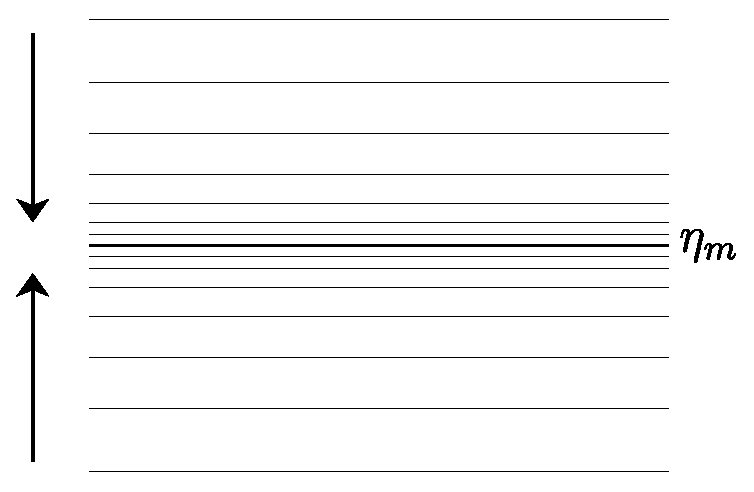
\includegraphics[width=80mm]{./Imagenes/densidad-eta-linea}}
            \hspace{1cm}
            \subfigure[Efecto de atracción al punto $(\xi_{n}, \eta_{n})$]{\label{fig:densidad-eta-punto}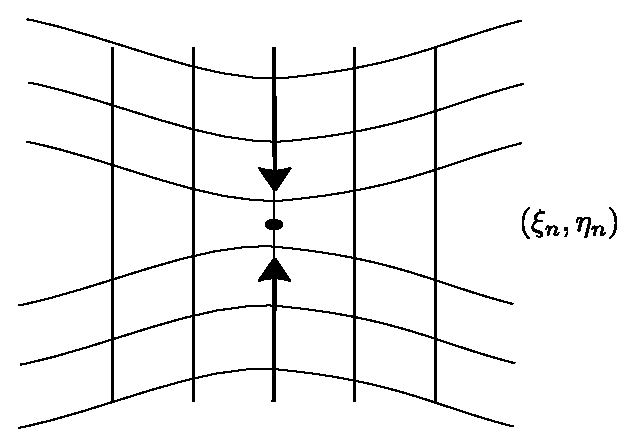
\includegraphics[width=80mm]{./Imagenes/densidad-eta-punto}}
            \caption[Efecto de atracción por función $Q(\xi,\eta)$]{Efecto de
            atracción en el eje $\eta$ por la función $Q(\xi, \eta)$}
            \label{fig:densidad-eta}
        \end{figure}
    \subsubsection{Generación de mallas mediante EDP hiperbólicas}
    \paragraph*{}
        La generación de mallas mediante EDP elípticas puede ser demasiado
        costosa en términos de tiempo de cómputo, así como en el uso de memoria
        en el ordenador. Esto se debe a que dicho esquema intenta hacer
        coincidir un sistema de coordenadas curvilíneo a cuatro curvas de
        frontera, seis en mallas tridimensionales. De aquí surge un nuevo
        enfoque, en el cual solo se requiere iniciar la solución con una sola
        frontera e ir avanzando hacia afuera en el dominio físico usando EDP
        hiperbólicas. \cite{farrashkhalvat}
    \paragraph*{}
        Con este propósito se toma en cuenta el trabajo publicado por Steger y
        Chausse \cite{Hyperbolic-steger1980generation} para la generación de
        mallas bidimensionales ortogonales y con control del área de celda. Se
        inicia el proceso con una frontera única en la que se considera que
        $\eta = 0$. Se propone tambien un sistema de ecuaciones de primer orden
        para las coordenadas $x, y$ como funciones de $\xi, \eta$:
        \begin{subequations}
            \begin{equation}
                g_{12} = g_1  \cdot g_2 = x_{\xi} x_{\eta} + y_{\xi} y_{\eta} = 0
            \end{equation}
            \begin{equation}
                \abs{g_1 \times g_2} = x_\xi y_\eta - x_\eta y_\xi = F
            \end{equation}
            \label{ec-hyper-base}
        \end{subequations}
    \paragraph*{}
        La primera ecuación dota a la malla de ortogonalidad, mientras que la
        segunda tiene el término $F$ como una medida del área de la celda (si el
        producto $\delta\xi\delta\eta$ es el mismo para cada celda). Se puede
        trabajar utilizando $F$ como una función de $\xi, \eta$, lo que
        permitiría incrementar la densidad de la malla cerca de la frontera
        donde $\eta = 0$ haciendo que $F$ tenga un valor pequeño en dicha zona.
        De las ecuaciones \ref{ec-hyper-base}:
        \begin{subequations}
            \begin{equation}
                x_\eta = - \frac{F}{ x_\xi ^ 2 + y_\xi ^ 2 } y_\xi
            \end{equation}
            \begin{equation}
                y_\eta = \frac{F}{ x_\xi ^ 2 + y_\xi ^ 2 } x_\xi
            \end{equation}
        \end{subequations}
    \paragraph*{}
        Antes de proceder a la solución del sistema de las ecuaciones
        \ref{ec-hyper-base} se deben tomar en cuenta algunas consideraciones. En
        primera instancia debe tenerse en cuenta que el sistema es un sistema no
        lineal por lo que un proceso de linearización debe llevarse a cabo, una
        segunda consideración es que al ser un sistema de ecuaciones
        hiperbólicas se debe llevar a cabo el proceso de solución mediante un
        proceso de marcha, en este trabajo la marcha se realizará en la
        dirección del eje $\eta$. Tercera, para un sistema de ecuaciones
        hiperbólicas se debe especificar una condicion inicial así como un
        condición de frontera y por último, con el objetivo de evitar la
        presencia de oscilaciones, se puede agregar un término de``damping'', o
        viscosidad artificial, al lado derecho de las ecuaciones.
    \paragraph*{}
        Para el proceso de linearización, se utilizará el esquema iterativo de
        Newton, el cual especifica que un termino no lineal es aproximado
        mediante
        \begin{equation}
            AB = A^{k + 1} B^{k} + B^{k + 1} A^{k} - A^{k} B^{k}
        \end{equation}
        donde el superíndice $k$ representa el estado previo conocido. A partir
        de este punto el superíndice $k + 1$, el cual representa el nivel actual
        a obtener, será eliminado de las ecuaciones, y se entiende que todos los
        términos sin superíndice pertenecen al nivel actual $k + 1$. Por lo
        tanto, el sistema de ecuaciones hiperbólicas es expresado en su forma
        lineal como:
        \begin{subequations}
            \begin{equation}
                x_{\xi} x_{\eta}^{k} + x_{\xi}^{k} x_{\eta} - x_{\xi}^{k} x_{\eta}^{k} + y_{\xi} y_{\eta}^{k} + y_{\xi}^{k} y_{\eta} - y_{\xi}^{k} y_{\eta}^{k} = 0
            \end{equation}
            \begin{equation}
                x_{\xi} y_{\eta}^{k} + x_{\xi}^{k} y_{\eta} - x_{\xi}^{k} y_{\eta}^{k} - x_{\eta} y_{\xi}^{k} - x_{\eta}^{k} y_{\xi} + x_{\eta}^{k} y_{\xi}^{k} = F
            \end{equation}
            \label{ec-hyper-linear}
        \end{subequations}
    \paragraph*{}
        Aplicando el concepto de las ecuaciones \ref{ec-hyper-base} a las
        ecuaciones \ref{ec-hyper-linear} podemos simplificar las últimas,
        quedando como
        \begin{subequations}
            \begin{equation}
                x_{\xi} x_{\eta}^{k} + x_{\xi}^{k} x_{\eta} + y_{\xi} y_{\eta}^{k} + y_{\xi}^{k} y_{\eta} = 0
            \end{equation}
            \begin{equation}
                x_{\xi} y_{\eta}^{k} + x_{\xi}^{k} y_{\eta} - x_{\eta} y_{\xi}^{k} - x_{\eta}^{k} y_{\xi} = F + F^{k}
            \end{equation}
            \label{ec-hyper-reducida}
        \end{subequations}
    \paragraph*{}
        Este sistema de ecuaciones puede escribirse de forma compacta como
        \begin{equation}
            \left[A \right] R_{\xi} + \left[ B \right] R_{\eta} = H
            \label{ec-hyper-compacta}
        \end{equation}\\ 
        donde:
        \begin{align*}
            R = \begin{bmatrix}
            x \\ \\
            y
            \end{bmatrix}&&
            A = \begin{bmatrix}
            x_{\eta}^{k} & y_{\eta}^{k} \\ \\
            y_{\eta}^{k} & -x_{\eta}^{k}
            \end{bmatrix}&&
            B = \begin{bmatrix}
            x_{\xi}^{k} & y_{\xi}^{k} \\ \\
            -y_{\xi}^{k} & x_{\xi}^{k}
            \end{bmatrix}&&
            H = \begin{bmatrix}
            0 \\ \\
            F + F^{k}
            \end{bmatrix}
        \end{align*}
    \paragraph*{}
        Por definición, el sistema de ecuaciones descrito por la ecuación
        \ref{ec-hyper-compacta} es hiperbólico si los eigenvalores de
        $\left[ B \right]^{-1} \left[ A \right]$ son reales. Se observa que\\
        \begin{equation*}
            \left[ B \right]^{-1} = \frac{1}{DN}\begin{bmatrix}
            x_{\xi}^{k} & -y_{\xi}^{k} \\ \\
            y_{\xi}^{k} & x_{\xi}^{k}
            \end{bmatrix}
        \end{equation*}\\
        por lo tanto
        \begin{equation*}
            \left[ C \right] = \left[ B \right]^{-1} \left[ A \right] = \begin{bmatrix}
            x_{\xi}^{k} x_{\eta}^{k} - y_{\xi}^{k} y_{\eta}^{k} &
            x_{\xi}^{k} y_{\eta}^{k} + x_{\eta}^{k} y_{\xi}^{k} \\ \\
            x_{\xi}^{k} y_{\eta}^{k} + x_{\eta}^{k} y_{\xi}^{k} &
            - \left( x_{\xi}^{k} x_{\eta}^{k} - y_{\xi}^{k} y_{\eta}^{k} \right)
            \end{bmatrix}
        \end{equation*}\\
        donde
        \begin{equation*}
            DN = \left( x_{\xi}^{k} \right)^2 + \left( y_{\xi}^{k} \right)^2
        \end{equation*}
    \paragraph*{}
        Los eigenvalores de $\left[ C \right]$ son
        \begin{equation*}
            \lambda_{1, 2} = \pm \left[ \frac{\left(x_{\eta}^{k} \right)^2 + \left( y_{\eta}^{k} \right)^2} {DN} \right]
        \end{equation*}\\
        los cuales cumplen con la condición de ser siempre reales (para un
        sistema hiperbólico) siempre que
        \begin{equation*}
            DN = \left( x_{\xi}^{k} \right)^2 + \left( y_{\xi}^{k} \right)^2 \neq 0
        \end{equation*}
    \paragraph*{}
        Para obtener un sistema de ecuaciones algebráico, debemos aplicar el
        método de diferencias finitas. Para la sustitución de las derivadas
        parciales respecto al eje $\xi$ se utiliza una aproximación central de
        segundo orden y para el caso de las derivadas parciales respecto al eje
        $\eta$ se hará uso de aproximaciones de primer orden tipo ``backwards'',
        resultando la ecuación en
        \begin{equation}
            \left[ A \right] \frac{R_{i + 1, j} - R_{i - 1, j}}{2 \Delta \xi} + \left[ B \right] \frac{R_{i, j} - R_{i, j - 1}}{\Delta \eta} = \left[ H \right]_{i, j}
        \end{equation}\\
        que al ser multiplicada por la matriz $\left[ B \right]^{-1}$ y reacomodada queda cómo
        \begin{equation}
            \frac{R_{i, j} - R_{i, j-1} }{\Delta \eta} + \left[ B \right]^{-1} \left[ A \right] \frac{R_{i + 1, j} - R_{i - 1, j} }{2 \Delta \xi} = \left[ B \right]^{-1} H_{i, j}
        \end{equation}\\
        en donde las matrices $A$ y $B$ son evaluadas en la línea $(j - 1)$.
        Esta ecuación se reacomoda y se le asignan nuevos términos, con el
        propósito de compactar a la misma, dando como resultado
        \begin{equation}
            \left[ AA \right] R_{i - 1, j} + \left[ BB \right] R_{i, j} + \left[ CC \right] R_{i + 1, j} = \left[ DD \right]_{i, j}
            \label{ec-hyper-final}
        \end{equation}\\
        donde
        \begin{subequations}
            \begin{equation*}
                \left[ AA \right] = - \frac{1}{2 \Delta \xi} \left[ C \right]_{i, j - 1}
            \end{equation*}
            \begin{equation*}
                \left[ BB \right] = \frac{1}{\Delta \eta} \left[ I \right]
            \end{equation*}
            \begin{equation*}
                \left[ CC \right] = \frac{1}{2 \Delta \xi} \left[ C \right]_{i, j - 1}
            \end{equation*}
            \begin{equation*}
                \left[ DD \right] = \left[ B \right]_{i, j - 1}^{-1} H_{i, j} + \frac{R_{i, j-1}}{\Delta \eta}
            \end{equation*}
        \end{subequations}\\
        una vez que se ha desarrollado la ecuación \ref{ec-hyper-final} para
        todas las instancias existentes a lo largo de $i$ para un mismo nivel
        $j$, se obtiene un sistema de bloque tridiagonal
        \begin{equation}
            \begin{bmatrix}
            \left[ BB \right]_2 & \left[ CC \right]_2 & & & & \\
            \left[AA\right]_3 & \left[BB\right]_3 & \left[CC\right]_3 & & & \\
            & \ddots & \ddots &  \ddots & & \\
            & & \ddots & \ddots & \ddots & & \\
            & & & \left[AA\right]_{m-2} & \left[BB\right]_{m-2} & \left[CC\right]_{m-2}\\
            & & & & \left[AA\right]_{m-1} & \left[BB\right]_{m-1}
            \end{bmatrix}
            \begin{bmatrix}
            R_{2}\\
            R_{3}\\
            \vdots\\
            \vdots\\
            R_{m-2}\\
            R_{m-1}
            \end{bmatrix}
            = \begin{bmatrix}
            \left[DD\right]_2\\
            \left[DD\right]_3\\
            \vdots\\
            \vdots\\
            \left[DD\right]_{m-2}\\
            \left[DD\right]_{m-1}
            \end{bmatrix}
        \end{equation}
        los términos $\left[DD\right]_2$ y $\left[DD\right]_{m - 1}$ son
        afectados por las condiciones de frontera de la siguiente manera
        \begin{subequations}
            \begin{equation*}
                \left[DD\right]_2 = \left[DD\right]_2 - \left[AA\right]_2 R_1
            \end{equation*}
            \begin{equation*}
                \left[DD\right]_{m - 1} = \left[DD\right]_{m - 1} - \left[CC\right]_{m - 1} R_{m}
            \end{equation*}
        \end{subequations}
    \paragraph*{}
        Este sistema de ecuaciones se resuelve avanzando en dirección del eje
        $\eta$, siempre y cuando la distribución de punto en la superficie y en
        las fronteras sea proporcionada.
    \paragraph*{}
        Los puntos en las fronteras deben ser libres de flotar, es decir, deben
        calcularse al final de cada iteración. Esto se logra aplicando la
        condición de ortogonalidad a las fronteras $i = 1$ e $i = m$ para
        actualizar dichos puntos.
    \paragraph*{}
        Un algoritmopara la solución de sistemas de ecuaciones de bloque
        tridiagonal es proporcionado en el apéndice \ref{appTridiagonal}
    \subsubsection{Generación de mallas mediante EDP parabólicas}
    \paragraph*{}
        El esquema elíptico desarrollado por Thompson et. al.
        \cite{thompson1974automatic} ha sido de los más utilizados en la
        generación de mallas estructuradas, sin embargo presenta ciertas
        desventajas que han hecho que se desarrollen otros enfoques y esquemas
        que sean más rápidos para obtener una solución y que consuman menos
        recursos computacionales. De este razonamiento surge el método propuesto
        por Steger y Chausse \cite{Hyperbolic-steger1980generation} el cual
        utiliza ecuaciones hiperbólicas para este propósito, entre las ventajas
        que dicho método presenta con respecto al esquema elíptico destaca el
        uso de un procedimiento de marcha lo que se traduce en un menor tiempo
        de ejecución del código dado que el esquema elíptico utiliza métodos
        iterativos y el tiempo de ejecución de un método de marcha es del orden
        que toma a un método iterativo llevar a cabo una iteración. Por otro
        lado, el usar ecuaciones hiperbólicas tiene a su vez desventajas como
        son la propagación de discontinuidades que puedan presentarse en la
        frontera interna conforme la solución marcha de dentro hacia afuera,
        otro punto importante de desventaja es que a menudo se necesita
        introducir términos que representen una ``viscosidad artificial'' en la
        solución ya que las soluciones de este tipo de ecuaciones tienden a ser
        inestables dadas sus caracterísitcas matemáticas. Por último, no es
        posible definir una frontera externa.
    \paragraph*{}
        En este trabajo se presenta el esquema desarrollado por Nakamura
        \cite{nakamuraParabolic} y que fue retomado por Siladic
        \cite{siladicParabolic}, el cual propone un método de generación de
        mallas a través de la solución de ecuaciones diferenciales parciales
        parabólicas. El uso de ecuaciones parabólicas presenta ciertas ventajas,
        entre ellas destaca el uso de métodos de solución de marcha, similares
        a los utilizados en la solución de ecuaciones hiperbólicas, dado que es
        una solución de problemas con condiciones iniciales, esto se traduce de
        igual manera en un tiempo de cómputo bajo. Por otro lado, las ecuaciones
        parabólicas comparten mucho del comportamiento matemático que está
        presente en las ecuaciones elípticas, que para el caso particular de la
        generación de mallas se traduce en el hecho de poseer un efecto difusivo
        que permite suavizar cualquier discontinuidad presente en la frontera
        interna conforme el procedimiento marcha de dentro hacia afuera. Por
        último, se posee la capacidad de definir las condiciones de frontera
        impuestas en la frontera externa.
    \paragraph*{}
        En resúmen, lo explicado arriba, es decir, el desarrollo de un algoritmo
        de generación de mallas mediante ecuaciones parabólicas tiene dos puntos
        de vital importancia, el primero de ellos es el bajo tiempo de ejecución
        computacional que es requerido para lograr la solución del problema, que
        representa una pequeña fracción del tiempo demandado por el esquema
        elíptico. El segundo es la baja demanda de memoria para llevar a cabo
        los cálculos requerido, y que además tambien es sustancialmente menor
        que el requerido por un esquema elíptico.
    \paragraph*{}
        Se propone el siguiente conjunto de ecuaciones
        \begin{subequations}
            \begin{equation}
                a(\xi, \eta) x_\eta = b(\xi, \eta)x_{\xi\xi} + c(\xi, \eta)V_x(\xi, \eta) + d(\xi, \eta)
            \end{equation}
            \begin{equation}
                a(\xi, \eta) y_\eta = b(\xi, \eta)y_{\xi\xi} + c(\xi, \eta)V_y(\xi, \eta) + d(\xi, \eta)
            \end{equation}
            \label{parabolic0}
        \end{subequations}\\
        donde $a, b$ y $c$ pueden ser constantes o alguna función de
        $(\xi,\eta)$, los valores $(x, y)$ representan las coordenadas en el
        dominio físico mientras quelos valores $(\xi, \eta)$ representan las
        coordenadas en el plano computacional, por último $V_x$ y $V_y$ son
        considerados términos fuente. En este esquema, la frontera externa se
        impone como una restricción sobre el comportamiento de la solución en la
        direccion $j$ mientras que la frontera interna funge como condición
        inicial del problema. Las ecuaciones \ref{parabolic0} son discretizadas
        mediante el método de diferencias finitas, las derivadas parciales con
        respecto al eje $\eta$ son sustituidas por aproximaciones tipo
        ``backwards'' mientras que las derivadas respecto al eje $\xi$ son
        reemplazadas por aproximanciones centrales. Dadas las condiciones
        inciales para $x$  y $y$ en $\eta = 0$, es decir, una vez proporcionada
        la nuve de puntos que definen la frontera interna, se obtiene un sistema
        de bloque tridiagonal, el cual debe ser resuelto para cada valor de
        $\eta$ contemplado.
    \paragraph*{}
        Los valores iniciales son especificados como:
        \begin{subequations}
            \begin{equation}
                x(\eta, 0) = x_0(\xi)
            \end{equation}
            \begin{equation}
                y(\eta, 0) = y_0(\xi)
            \end{equation}
        \end{subequations}\\
        donde $x_0(\xi)$ y $y_0(\xi)$ las coordenadas de la superficie de la
        frontera, es decir, del perfil aerodinámico a analizar. Para entender el
        efecto de los términos fuente, se asigna un valor cero a las constantes
        $b$ y $c$, a su vez $a = c = 1$, expresando las ecuaciones resultantes
        en términos de incrementos en lugar de términos diferenciales:
        \begin{subequations}
            \begin{equation}
                \Delta x = V_x(\xi, \eta) \Delta \eta
            \end{equation}
            \begin{equation}
                \Delta y = V_y(\xi, \eta) \Delta \eta
            \end{equation}
            \label{source-effect}
        \end{subequations}\\
        en las ecuaciones \ref{source-effect} se observa que conforme $\eta$
        aumenta, el cambio tanto en $x$ como en $y$ está determinado por $V_x$
        y $V_y$ respectivamente, lo que implica que ambos términos fuente deben
        especificarse de tal modo que $x$ y $y$ aumenten en la dirección y
        magnitud deseados. Por otro lado, las segundas derivadas parciales
        $x_{\xi\xi}$ y $y_{\xi\xi}$ en las ecuaciones \ref{parabolic0} tienen un
        efecto disipador para los intervalos en dirección $\xi$. Los valores de
        los términos fuente $V_x$ y $V_y$ pueden ser determinados mediante
        interpolación, ya sea polinomial o lineal, entre las fronteras interna y
        externa. Si se desea tener un control sobre la ortogonalidad del
        mallado, es posible la introducción de una frontera falsa para la
        frontera externa que permita lograr dicha característica, sumado a esto,
        es posible variar la distancia entre nodos en ambas direcciones $\xi$ y
        $\eta$ al discretizar las ecuaciones \ref{parabolic0} sobre una malla no
        uniforme en el plano computacional.
    \paragraph*{}
        En la mayoría de casos, y en general en la literatura encontrada en la
        generación de mallas, se asume una malla uniforme y en algunos casos se
        sugiere que el espacio entre nodos sea igual a la unidad, esto último
        con el objetivo de simplificar las ecuaciones. Sin embargo, estas
        consideraciones no son estrictamente necesarias sino que representan
        simplificaciones del problema, por lo que la generación de una malla
        cuasi uniforme en el plano computaciones, y que despues se utilice en el
        anáñlisis de flujos como si de una malla uniforme se tratase, es tambien
        un enfoque válido.
        \begin{figure}[htbp!]
            \centering
            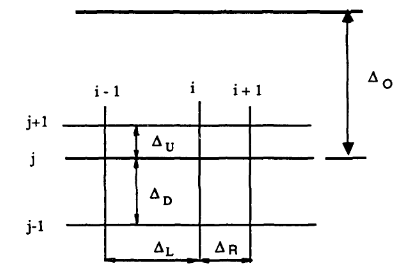
\includegraphics[width=100mm]{./Imagenes/parabolic_non_uniform.png}
            \caption[Generación de malla cuasi uniforme por ecuaciones
            parabólicas]{Generación de malla estructurada cuasi uniforme
            desarrollada mediante ecuaciones parabólicas \cite{siladicParabolic}}
            \label{fig:parabolic_non_uniform}
        \end{figure}
    \paragraph*{}
        En la figura \ref{fig:parabolic_non_uniform} se muestra un ejemplo de
        malla no uniforme, donde $\Delta L$ y $\Delta R$ representan incrementos
        en la dirección $i$, a su vez $\Delta U$ y $\Delta D$ representan
        incrementos en términos de $j$ para un punto $(i, j)$ dado. Retomando lo
        expuesto en el capítulo \ref{chap:discretizacion-espacial}, se pueden
        usar series de Taylor para aproximar los términos que incluyen derivadas
        en las ecuaciones gobernantes en el esquema parabólico, quedando de la
        siguiente manera:
        \begin{align*}
            f_x = \frac{f_{i+1, j} - f_{i,j}}{\Delta R} && y && f_x = \frac{f_{i, j} - f_{i-1, j}}{\Delta L}\\
            f_y = \frac{f_{i, j+1} - f_{i,j}}{\Delta U} && y && f_y = \frac{f_{i, j} - f_{i, j-1}}{\Delta D}
        \end{align*}
        \begin{align*}
        f_{xx} = \frac{2}{\Delta R + \Delta L} \left( \frac{f_{i+1, j} - f_{i,j}}{\Delta R} - \frac{f_{i, j} - f_{i-1, j}}{\Delta L} \right)\\
        f_{yy} = \frac{2}{\Delta D + \Delta U} \left( \frac{f_{i, j+1} - f_{i,j}}{\Delta U} - \frac{f_{i, j} - f_{i, j-1}}{\Delta D} \right)\\
        f_{xy} = \frac{f_{i+1,j+1} - f_{i+1, j-1} - f_{i-1, j+1} + f_{i-1, j-1}}{\left( \Delta R + \Delta L \right) \left( \Delta D + \Delta U \right)}
        \end{align*}\\
        con esto, las ecuaciones gobernantes \ref{parabolic0} se discretizan de
        la siguiente manera
        \begin{subequations}
            \begin{equation}
            \frac{a \left( x_{i,j} - x_{i, j-1} \right)}{\Delta D} = \frac{2b}{\Delta L + \Delta R} \left[ \frac{x_{i+1, j} - x_{i, j}}{\Delta R}  - \frac{x_{i, j} - x_{i-1, j}}{\Delta L} \right] + c \frac{XB_{i, Jmax} - x_{i, j}}{\Delta O} + d
            \end{equation}
            \begin{equation}
            \frac{a \left( y_{i,j} - y_{i, j-1} \right)}{\Delta D} = \frac{2b}{\Delta L + \Delta R} \left[ \frac{y_{i+1, j} - y_{i, j}}{\Delta R}  - \frac{y_{i, j} - y_{i-1, j}}{\Delta L} \right] + c \frac{YB_{i, Jmax} - y_{i, j}}{\Delta O} + d
            \end{equation}
            \label{parabolic1}
        \end{subequations}
    \paragraph*{}
        Para poder determinar los valores de los coeficientes $a$, $b$ y $c$ y
        para entender el método presente para el control de la densidad de
        mallado, se deben relacionar las ecuaciones gobernantes con un conjunto
        de ecuaciones conocidas en el plano computacional. Con este propósito es
        que se seleccionan las ecuaciones de Laplace en el modelo de generación
        de mallas mediante ecuaciones elípticas (ecuaciones
        \ref{ec-laplace-invertida}), intentando obtener un método equivalente al
        obtenido en el esquema elíptico, en el que cualquier línea $m$ en la
        dirección $\eta$ sea forzada a moverse hacia una línea $m - 1$. En la
        figura \ref{fig:eliptic_non_uniform} se muestra un representación de lo
        descrito, siendo para un punto $(i, j)$, $F_{i-1}$ y $F_i$ incrementos
        en la dirección $\xi$ y a su vez $g_{j-1}$ y $g_j$ incrementos en la
        dirección $\eta$.\\
        \begin{figure}[htbp!]
            \centering
            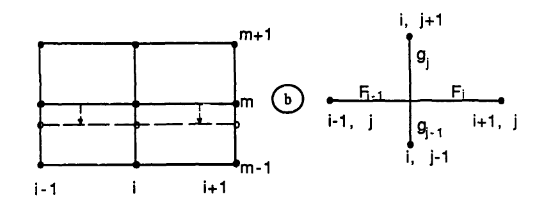
\includegraphics[width=110mm]{./Imagenes/eliptic_non_uniform.png}
            \caption[Generación de malla por ecuaciones elípticas]{Generación de
            malla estructurada no uniforme desarrollada mediante ecuaciones
            elípticas \cite{siladicParabolic}}
            \label{fig:eliptic_non_uniform}
        \end{figure}
    \paragraph*{}
        Las ecuaciones del modelo de generación de mallas elíptico (ecuaciones
        \ref{ec-laplace-invertida}), bajo este nuevo esquema basado en la
        generación de una malla cuasi uniforme se discretizan en $(\xi, \eta)$
        dando como resultado
        \begin{align}
            &\begin{aligned}
                &&\frac{2\alpha}{F_i + F_{i - 1}} \left[ \frac{s_{i-1, j} - s_{i, j}}{F_{i - 1}} + \frac{s_{i+1, j}  - s_{i, j}}{F_i} \right] + \beta \left[ \frac{ s_{i+1, j+1} - s_{i+1, j-1} - s_{i-1, j + 1} + s_{i-1, j-1} }{ (F_{i - 1} + F_i) (g_{j - 1} + g_j) } \right]\\&& + \frac{2\gamma}{g_j + g_{j - 1}} \left[ \frac{s_{i, j-1} - s_{i, j}}{g_{j - 1}}  + \frac{s_{i, j+1} - s_{i, j}}{g_j}\right] = 0
            &\end{aligned}
            \label{eliptic_non_uniform}
        \end{align}
    \paragraph*{}
        A partir de la ecuación \ref{eliptic_non_uniform} se propone un
        procedimiento de marcha, reemplazando en dicha ecuación los valores
        $x_{i, j + 1}$ y $y_{i, j+1}$ por valores conocidos $XO_{i, j + 1}$ y
        $YO_{i, j + 1}$ los cuales son obtenidos mediante interpolación lineal
        entre los valores de la frontera interna (perfil aerodinámico) y la
        frontera externa (tipología de la malla). La distancia $g_j$ puede
        cambiarse gradualmente a lo largo de la malla para una mayor
        versatilidad en la generación de la ésta.
    \paragraph*{}
        En el caso más sencillo, aquel en el que no interesa forzar la
        ortogonalidad en las fronteras, a las variables $XO$ y $YO$ se les
        asignan los valores $(XB_{i, Jmax} YB_{i, Jmax})$ en la frontera
        externa. Reordenando los términos, y donde $s$ representa cualquier
        coordenada $x$ o $y$\\
        \begin{align}
            \begin{aligned}
                \frac{2\alpha}{F_i + F_{i - 1}} \left[ \frac{s_{i-1, j} - s_{i, j}}{F_{i - 1}} + \frac{s_{i+1, j} - s_{i, j}}{F_i} \right] + \frac{2\gamma}{g_{j - 1} + G_j} \left[ \frac{-s_{i, j}}{g_{j - 1}} - \frac{s_{i, j}}{G_j} \right]\\
                = -\beta \left[ \frac{ SO_{i+1, j+1} - SO_{i-1, j-1} - s_{i+1, j-1} + s_{i-1, j-1} }{ (F_{i - 1} + F_i) (g_{j - 1} + G_j) } \right] - \frac{2\gamma}{g_{j-1} + G_j} \left[ \frac{s_{i, j - 1}}{g_{j - 1}} + \frac{SO_{i, j + 1}}{G_j} \right]
            \end{aligned}
            \label{eliptic_non_uniform1}
        \end{align}\\
        donde
        \begin{align*}
            &\begin{aligned}
            G_j = g_j + g_{j + 1} + ... + g_{Jmax - 1} = \eta_{max} - \eta_j
            \end{aligned}\\
            &\begin{aligned}
            g_{j - 1} = \eta_j - \eta_{j - 1};&& F_i = \xi_{i + 1} - \xi_i; && F_{i - 1} = \xi_i - \xi_{i - 1}&&
            \end{aligned}
        \end{align*}\\
        $G_j$ representa la distancia entre las líneas $(i, j)$ e $(i, JO)$ en
        el plano computacional, por lo tanto $SO_{i, j} = XO_{i, j}$ o
        $YO_{i, j}$. Si comparamos ambos modelos discutidos en esta sección, es
        decir el modelo parabólico (ecuaciones \ref{parabolic1}) y el modelo
        elíptico (ecuaciones \ref{eliptic_non_uniform1}) se puede establecer una
        clara relación, al colocar de un lado las incógnitas de cada ecuación, y
        del otro todos los valores conocidos, es decir
        \begin{align}
            \begin{aligned}
                -\left( \frac{b}{\Delta L} + \frac{b}{\Delta R} \right) \frac{2 s_{i, j}}{\Delta L + \Delta R} &- \left( \frac{a}{\Delta D} + \frac{c}{\Delta O}\right) s_{i, j} + \frac{b}{\Delta R} \frac{2 s_{i-1, j}}{\Delta R + \Delta L} + \frac{b}{\Delta R} \frac{2 s_{i+1, j}}{\Delta R + \Delta L}\\
                &= - c \frac{SB_{i, Jmax}}{\Delta O} - a \frac{s_{i, j-1}}{\Delta D} - d
            \end{aligned}
        \end{align}
        \begin{align}
            \begin{aligned}
                -\left( \frac{\alpha}{F_{i - 1}} + \frac{\alpha}{F_i} \right) \frac{2s_{i, j}}{F_i + F_{i - 1}} - \left( \frac{\gamma}{g_{j - 1}} + \frac{\gamma}{G_j} \right) \frac{2s_{i, j}}{G_j + g_{j-1}} + \frac{\alpha}{F_{i - 1}} \frac{2 s_{i-1, j}}{F_i + F_{i - 1}} + \frac{\alpha}{F_i} \frac{2 s_{i, j}}{F_i + F_{i - 1}}\\
                = - \frac{2\gamma}{g_{j - 1} + G_j} \left[ \frac{SO_{i, j+1}}{G_j} + \frac{s_{i, j-1}}{g_{j -1}} \right] - \beta \left[ \frac{SO_{i+1, j+1} - SO_{i-1, j+1} - s_{i+1, j-1} + s_{i-1, j-1} }{ \left( F_i + F_{i - 1} \right) \left( g_{j - 1} + G_j \right) } \right]
            \end{aligned}
        \end{align}\\
        de este reacomodo se puede observar que ambas ecuaciones tienen la misma
        forma, por lo que es posible establecer una relación entre sus
        coeficientes\\
        \begin{subequations}
            \begin{equation*}
                b = \alpha
            \end{equation*}\\
            \begin{equation*}
                a = c = \frac{2\gamma}{G_j + g_{j - 1}}
            \end{equation*}\\
            \begin{equation*}
                d = \beta \left[ \frac{SO_{i+1, j+1} - SO_{i-1, j+1} - s_{i+1, j-1} + s_{i-1, j-1} }{ (F_i + F_{i-1}) (G_j + g_{j-1}) } \right]
            \end{equation*}
        \end{subequations}\\
        donde $\alpha$, $\beta$ y $\gamma$ son los coeficientes de las
        ecuaciones \ref{ec-laplace-invertida}. El sistema representado por la
        ecuación \ref{eliptic_non_uniform1} representa un sistema tridiagonal de
        matrices $2$x$2$ el cual se desarrolla del siguiente modo\\
        \begin{align*}
            &\begin{aligned}
                &&&&&&&&&&&&&&&&&&A = \frac{2\alpha}{F_{i - 1} (F_i + F_{i - 1}) } &&& ; &&& C =& \frac{2\alpha}{F_i (F_i + F_{i - 1}) }
            \end{aligned}\\ \\
            &\begin{aligned}
                &&&&&&&&&&&&&&&B = \frac{-2 \alpha}{F_i + F_{i - 1}} \left( \frac{1}{F_i} + \frac{1}{F_{i - 1}} \right) - \frac{2\gamma}{G_j + g_{j - 1}} \left( \frac{1}{G_j}  + \frac{1}{g_{j - 1}} \right)
            \end{aligned}\\ \\
            &\begin{aligned}
                D_x = -\beta \frac{ XO_{i+1, j+1} - XO_{i-1, j+1} - x_{i+1, j-1} + x_{i-1, j-1} }{ (F_i + F_{i - 1}) (G_j + g_{j - 1}) } - \frac{2 \gamma}{G_j + g_{j - 1}} \left[ \frac{x_{i, j - 1}}{g_{j-1}} + \frac{XO_{i, j + 1}}{G_j} \right]
            \end{aligned} \\ \\
            &\begin{aligned}
                D_y = -\beta \frac{ YO_{i+1, j+1} - YO_{i-1, j+1} - y_{i+1, j-1} + y_{i-1, j-1} }{ (F_i + F_{i - 1}) (G_j + g_{j - 1}) } - \frac{2 \gamma}{G_j + g_{j - 1}} \left[ \frac{y_{i, j - 1}}{g_{j-1}} + \frac{YO_{i, j + 1}}{G_j} \right]
            \end{aligned}
        \end{align*}\\
        finalmente, las ecuaciones gobernantes del sistema parabólico pueden
        expresarse como:\\
        \begin{subequations}
            \begin{equation}
                Ax_{i-1, j} + B x_{i, j} + Cx_{i+1, j} = D_x
            \end{equation}
            \begin{equation}
                Ay_{i-1, j} + B y_{i, j} + Cy_{i+1, j} = D_y
            \end{equation}
            \label{parabolic_final}
        \end{subequations}
    \paragraph*{}
        Las ecuaciones \ref{parabolic_final} se resuelven simultaneamente para
        todos los puntos de la malla para el mismo nivel $\eta$ (línea $j$)
        resolviendo el sistema tridiagonal para cada $x_{i, j}$ y $y_{i, j}$. La
        solución comienza en $j = 1$ (justo después de la frontera interna) y
        finaliza en $j = Jmax - 2$ (un nivel antes de la frontera externa). Los
        coeficientes $\alpha$, $\beta$ y $\gamma$ se calculan usando las
        coordenadas de puntos adyacentes que ya se han generado, dichos valores
        son sustituidos en las aproximaciones por diferencias finitas utilizadas
        para reemplazar las primeras derivadas parciales, las cuales para este
        sistema quedan expresadas como\\
        \begin{subequations}
            \begin{equation}
                x_\xi = \frac{x_{i+1, j-1} - x_{i-1, j-1}}{F_i + F_{i-1}}
            \end{equation}
            \begin{equation}
                y_\xi = \frac{y_{i+1, j-1} - y_{i-1, j-1}}{F_i + F_{i-1}}
            \end{equation}
            \begin{equation}
                x_\eta = \frac{XO_{i, j+1} - x_{i, j-1}}{g_{j-1} + G_j}
            \end{equation}
            \begin{equation}
                y_\eta = \frac{YO_{i, j+1} - y_{i, j-1}}{g_{j-1} + G_j}
            \end{equation}
        \end{subequations}
    \paragraph*{}
        Los términos no uniformes en la separación de la malla descritos arriba
        tienen un efecto similar al control de la densidad de mallado mediante
        funciones exponenciales presentado por Thompson, Thames y Mastin
        \cite{thompson1974automatic} para la generación de mallas mediante el
        esquema elíptico.
    \paragraph*{Ortogonalidad de la Malla}
    \paragraph*{}
        ``Al analizar y resolver flujos viscosos o capas límite, la
        ortogonalidad de las líneas de la malla en las cercanías a las
        superficies de cuerpos es deseable para representar todas las derivadas
        normales de manera simple y  precisa''\cite{siladicParabolic}. Si se
        desea lograr esto, se debe tener la capacidad de controlar la
        orientación de las líneas, lo cual puede lograrse introduciendo una
        frontera externa modificada lo que permite determinar los valores de los
        términos fuente. Es decir, si la frontera externa modificada se
        posiciona de manera que sus puntos se localizen perpendicularmente a sus
        correspondientes sobre la superficie del cuerpo, las líneas se alejarán
        del cuerpo de manera ortogonal. Esto es mejor ilustrado en la figura
        \ref{fig:parabolic_modified}.
        \begin{figure}[htbp!]
            \centering
            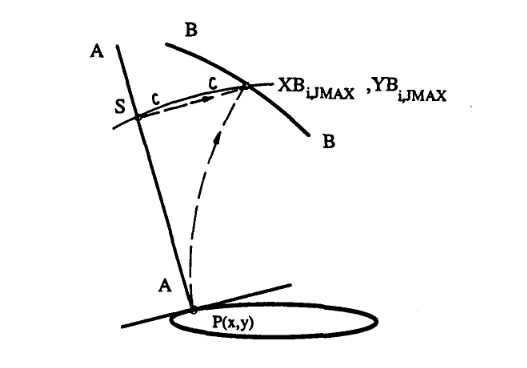
\includegraphics[width=110mm]{./Imagenes/parabolic_modified_boundary.png}
            \caption[Control de ortogonalidad]{Control de ortogonalidad en la
            generación de mallas por ecuaciones parabólicas \cite{siladicParabolic}}
            \label{fig:parabolic_modified}
        \end{figure}
    \paragraph*{}
        Si nos ubicamos en un punto $(i, j)$ con sus correspondientes
        coordenadas $(XO_{i, j + 1}, YO_{i, j+1})$, se observa de la figura
        \ref{fig:parabolic_modified} una recta $AA$ que es perperndicular a la
        superficie de la frontera interna la cual nace del punto $(i, 0)$, punto
        que corresponde a la misma línea $\xi = cte$ del punto en el que nos
        ubicamos. También podemos observar en la figura un arco de
        circunferencia $CC$, dicho arco tiene su centro en el punto $(i, 0)$ y
        pasa por las coordenadas $(XB_{i, Jmax}, YB_{i, Jmax})$ de la frontera
        externa no modificada. La intersección de la línea $AA$ y del arco $CC$
        representa los valores dados para las coordenadas $(XO_{i, j + 1},
        YO_{i, j+1})$ con el uso de una frontera modificada.
    %
    %
    %
    %
    %

    %
    %
    %
    %
    %
\chapter{Desarrollo Práctico}
    \paragraph*{}
        Los códigos de este trabajo fueron implementados en lenguaje Python 3,
        utilizando el paradigma de programación orientada a objetos, en éste los
        datos son trabajados como objetos con atributos y métodos pertenecientes
        a una clase, y que pueden ser heredados y aplicados a objetos o
        instancias de alguna subclase. Un objeto  es la representación en un
        programa de un concepto y contiene toda la información necesaria para
        abstraerlo, como son los datos que describen sus atributos y operaciones
        que pueden realizarse dobre los mismos.  En otras palabras un objetos es
        la relación que existe entre un conjunto de variables y métodos.
    \paragraph*{}
        Se dice que todos las instancias (objetos) de un mismo tipo, son
        pertenecientes a una misma clase. Una de las características más
        importantes de la programación orientada a objetos es la herencia, la
        cual permite la definición de nuevas clases a partir de una
        ``superclase'' ya existente, las cuales se conocen como ``subclases''.
        Una subclase hereda todo el comportamiento de su superclase, pero se
        puede introducir además características propias.
    \paragraph*{}
        En el presente trabajo se implementaron dos superclases: ``airfoil'' y
        ``mesh'', cada una con sus respectivas subclases.
        La clase airfoil se desarrolló para la creación de perfiles alares a
        partir de una archivo de texto que contenga la nube de puntos del perfil
        deseado, como dato de entrada se requiere el nombre del archivo texto y
        la dimensión en metros de la cuerda. Esta clase tiene una subclase
        ``NACA4'' la cual genera perfiles de la serie de 4 dígitos de perfiles
        aerodinámicos de la NACA. La creación del perfil se hace a partir de la
        ecuación constitutiva de la serie. Como datos de entrada se requieren
        los valores de m (combudara máxima), p (posición de la combadura
        máxima), t (espesor máximo) y c (cuerda). La subclase NACA4 tiene dos
        métodos para la creación del perfil, el primero de ellos, el método
        ``create\textunderscore linear'' crea la nube de puntos con una
        distribución equidistante de los puntos en dirección del eje $x$.
        El segundo método, llamado ``create\textunderscore sin''genera a partir
        de una función senoidal una nube de punto que permite que haya mayor
        densidad de nodos tanto en el borde de ataque como en el borde de salida
        del perfil.
%
%
%
%
%

\chapter{Análisis de Flujo Potencial}
    \paragraph*{}
        El modelo de flujo potencial es la más simple consideración de flujo no viscoso en
        tomar en cuenta los efectos de compresibilidad.

    \paragraph*{}
        Para el caso de flujos externos, en este caso el flujo de una corriente
        de aire alrededor de un perfil aerodinámico, existen ciertas
        consideraciones que permiten tratar el flujo como no viscoso e
        irrotacional.

    \paragraph*{}
        Se sabe que la condición de irrotacionalidad requiere la ausencia de
        viscosidad, así como de gradientes de velocidad en la dirección normal
        al flujo. Teoricamente estas condiciones en el flujo son imposibles de
        conseguir, sin embargo en flujos de fluidos con valores relativamente
        pequeños de viscosidad (como el agua y el aire) los efectos de la capa
        límite suceden en una sección en teoría demasiado pequeña, con lo  que
        dicha sección puede ser despreciada durante el análisis. En cuanto al
        resto del flujo, la condición de irrotacionalidad, así como la no
        consideración de los efectos viscosos, son simplifaciones válidas.

    \paragraph*{}
        Como ya se mencionó, la condición principal que debe tener el flujo
        para poder ser considerado potencial y no viscoso es la
        irrotacionalidad. De acuerdo al teorema de Kelvin, si el flujo es
        irrotacional en un momento, continuara siendo irrotacional y por lo
        tanto también será isentrópico.

    \paragraph*{}
        Estas consideraciones teóricas llevan consigo una serie de
        simplificaciones a las ecuaciones de Navier Stokes que facilitan el
        análisis de diversos flujos. En primera instancia, al decirse que el
        flujo es no viscoso se debe despreciar los efectos de los esfuerzos
        cortantes, dicha simplificación nos permite trabajar con las ecuaciones
        de Euler. Si además de esto, se toma como irrotacional el flujo, se
        obtienen las ecuaciones de Bernoulli.

    \paragraph*{}
        Para flujos no viscosos, la función de potencial puede definirse
        como:
        \begin{equation}
            \vec{v} = \vec{\nabla} \phi
            \label{u_eq_phi}
        \end{equation}
        La forma conservativa de la ecuación del potencial puede obtenerse a
        partir de la ecuación de la continuidad.
        \begin{equation}
            \pdv{\rho}{t} + \vec{\nabla} \cdot \left( \rho \vec{\nabla} \phi \right) = 0
        \end{equation}

    \paragraph*{}
        La ecuación de momento y energía pueden reducirse a la siguiente
        ecuación para la entalpía de estancamiento:
        \begin{equation}
            \pdv{\phi}{t} + H = H_{0}
        \end{equation}
        donde $H_0$ representa la entalpía de estancamiento y es un valor constante para todo el fluido.

    \paragraph*{}
        La densidad es una función tanto de $\vec{\nabla} \phi$ como de
        $\pdv{\phi}{t}$, que para el caso de un gas perfecto (dado que el
        flujo potencial se considera isentrópico) con valores
        definidos para la densidad y entalpía de estancamiento $\rho_{0}$
        y $H_{0}$ se escribe como:
        \begin{equation}
            \frac{\rho}{\rho_{0}} = \left[ 1
                - \frac{(\vec{\nabla} \phi) ^ 2}{2 H_0}
                - \frac{\pdv{\phi}{t}}{H_0} \right]^{\frac{1}{\gamma - 1}}
        \end{equation}

    \paragraph*{}
        Para el caso de un flujo estacionario la ecuación del flujo potencial
        resulta:
        \begin{equation}
            \vec{\nabla} \cdot \left( \rho \vec{\nabla} \phi \right) = 0
            \label{stationary_flow}
        \end{equation}

        mientras que la ecuación de la energía, a través de las relaciones
        para gas isentrópico, queda como
        \begin{equation}
            H \equiv h + \frac{\vec{v}^2}{2} = H_0
        \end{equation}

    \paragraph*{}
        Dada una transformación de sistemas coordenados como la descrita en
        capítulos anteriores:
        \begin{align*}
            \xi = \xi(x, y)
            \\
            \eta = \eta(x, y)
        \end{align*}
        la ecuación de flujo potencial puede ser escrita como
        \begin{equation}
            \pdv{t} \left( \frac{\rho}{J} \right) + \pdv{\xi} \left( \rho
                    \frac{U}{J} \right) + \pdv{\eta} \left( \rho \frac{V}{J}
                        \right) = 0
        \end{equation}

    \paragraph*{}
        Las componentes de la velocidad en el dominio computacional $U$ y $V$
        pueden definirse en función de las componentes del sistema cartesiano
        $u$ y $v$ como:
        \begin{subequations}
            \begin{equation}
                U = \xi_{x} \phi_{x} + \xi_{y} \phi_{y}
                        = \xi_{x} u + \xi_{y} v
            \end{equation}
            \begin{equation}
                V = \eta_{x} \phi_{x} + \eta_{y} = \eta_{x} u + \eta_{y} v
            \end{equation}
        \end{subequations}

    \paragraph*{}
        A partir de las ecuaciones \ref{u_eq_phi} y \ref{stationary_flow} se
        puede obtener una ecuacion para flujo potencial estacionario
        \begin{equation}
            \vec{\nabla} \cdot \left( \rho \vec{v} \right)
                    = \pdv{\xi} \left[ \left(g^{11}\phi_{\xi}
                            + g^{12} \phi_{\eta} \right) \frac{\rho}{J} \right]
                        + \pdv{\eta} \left[ \left(g^{21} \phi_{\xi}
                            + g^{22} \phi_{\eta} \right) \frac{\rho}{J} \right]
                    = 0
        \end{equation}
        ya que tambien se tiene:
        \begin{align}
            U = g^{11} \phi_{\xi} + g^{12} \phi_{\eta}
            \\
            V = g^{21} \phi_{\xi} + g^{22} \phi_{\eta}
        \end{align}

    \paragraph*{}
        A su vez la matriz del tensor de la transformación $[g]$ tiene las
        siguientes componentes
        \begin{subequations}
            \begin{equation}
                g^{11} = \xi_{x}^{2} + \xi_{y}^2
            \end{equation}
            \begin{equation}
                    g^{12} = g^{21} = \xi_{x} \eta_{x} + \xi_{y} \eta_{y}
            \end{equation}
            \begin{equation}
                g^{22} = \eta_{x}^{2} + \eta_{y}^2
            \end{equation}
        \end{subequations}

    \paragraph*{}
        En la mayoría de los flujos de análisis práctico, es generalmente
        necesario trabajar con la transformación inversa:
        \begin{subequations}
            \begin{equation}
                x = x \left( \xi, \eta \right)
            \end{equation}
            \begin{equation}
                y = y \left( \xi, \eta \right)
            \end{equation}
        \end{subequations}
    \\ la cual es obtenida a traves de las transformaciones
    \begin{align}
        \xi_{x} = J y_{\eta} && \xi_{y} = -J x_{\eta}
        \\
        \eta_{x} = -J y_{\xi} && \eta_{y} = J x_{\xi}
    \end{align}
    \\ con el Jacobiano
    \begin{equation}
        J = \frac{1}{x_{\xi} y_{\eta} - x_{\eta} y_{\xi}}
    \end{equation}

    \section{Condiciones de Frontera}
    \paragraph*{}
        Para que una simulación se lleve a cabo es necesario establecer un
        dominio computacional, el cual contará con una o más fronteras
        $\Gamma$, sobre dichas fronteras se deben especificar las
        correspondientes condiciones de frontera que dotarán de sentido físico
        a la simulación, es decir, para este caso se deben especificar
        condiciones de frontera que coincidan con la teoría de flujo potencial.

    \subsection{Condiciones en las lejanías}
    \paragraph*{}
        En la frontera externa el campo de fluido se asume como conocido. Para
        casos de flujos externos, como lo es el caso de un perfil inmerso en un
        flujo uniforme con velocidad $\vec{V}_{\infty}$, el flujo potencial
        está definido mediante:
        \begin{equation}
            \phi = \vec{V}_{\infty} \cdot \vec{x} + \phi_{0}
        \end{equation}
        donde $\phi_{0}$ es una constante arbitraria y $\vec{x}$ representa
        la distancia a un punto de la frontera con respecto a una referencia
        establecida previamente.

    \paragraph*{}
        Para cuerpos que producen sustentación con una circulación $\Gamma_{B}$,
        se debe tomar en cuenta la contribución de dicha circulación al flujo
        potencial en una distancia lejana. En el caso de perfil bidimensionales
        esto se logra mediante la adición de un vórtice, corregido por efectos
        de compresibilidad:
        \begin{equation}
            \phi_{\infty} = \vec{V}_{\infty} \cdot \vec{x}
                            + \frac{\Gamma_B}{2 \pi} \tan^{-1}
                                \left[ \sqrt{1-M_{\infty}^{2}}
                                tan(\theta - \alpha_{\infty}) \right] + \phi_{0}
        \end{equation}
        donde $\theta$ es la posición angular de un punto en la lejanía,
        $\Gamma_B$ es la circulación y $M_\infty$ es el número de Mach
        correspondiente a la velocidad de la corriente libre $\vec{V}_\infty$
        con un ángulo de incidencia $\alpha_{\infty}$.

        \begin{figure}[htbp!]
            \centering
            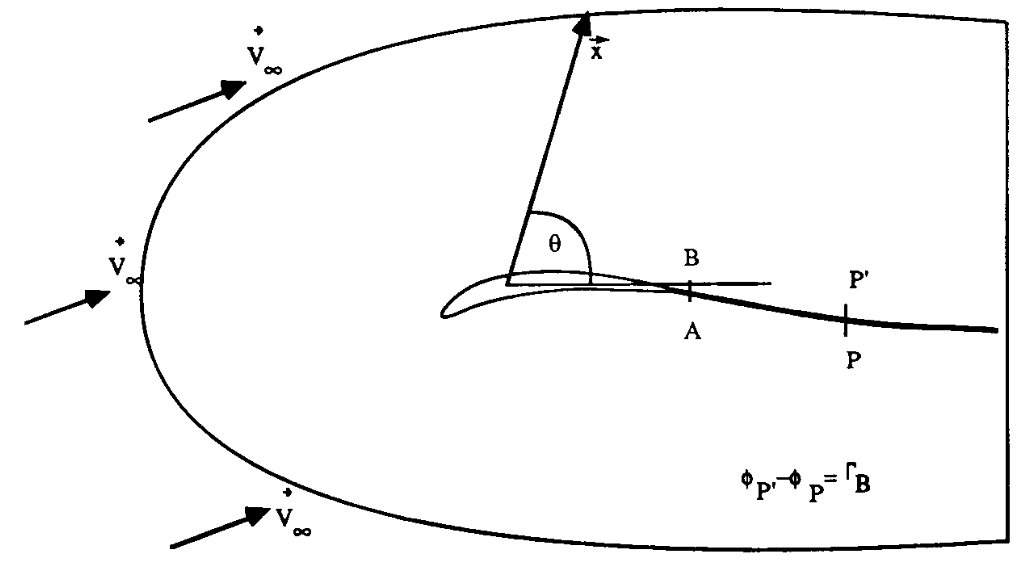
\includegraphics[width=115mm]{./Imagenes/circulacion_phi}
            \caption[Condiciones de frontera de flujo potencial]{Condiciones de
                frontera de flujo potencial para perfil aerodinámico
                bidimensional\cite{potential_flow}}
            \label{phi_circulacion_malla}
        \end{figure}

    \subsection{Condiciones para perfiles aerodinámicos}
    \paragraph*{}
        Los perfiles aerodinámicos requieren una circulación cuya intensidad es
        definida por la condición de Kutta. En simulaciones computacionales un
        ``corte" debe definirse, a lo largo del cual existirá una discontinuidad
        del potencial dado por
        \begin{equation}
            \phi_{P'} - \phi_{P} = \Gamma_{B} = \phi_{B} - \phi_{A}
        \end{equation}

    \paragraph*{}
        El valor de la circulación debe ser actualizado en cada iteración del
        proceso de solución, esto se logra imponiendo velocidades o presiones
        iguales en ambos lados del borde de salida.

    \section{Discretización para flujo subsonico estacionario}
    \paragraph*{}
        La ecuación de flujo potencial en su variable estacionaria para flujo
        subsonico es una ecuación diferencial parcial elíptica. Esto presenta la
        facilidad de utilizar diferencias finitas como método de discretización
        del problema, sin embargo es importante recalcar que este no es el
        único método válido y que tambien es posible llevar a cabo la
        discretización mediante los métodos de volumenes y elementos finitos.

    \paragraph*{}
        Ya que los flujos subsónicos presentan generalmente un comportamiento
        ``suave" es posible realizar las simulaciones con mallas que tengan una
        alta densidad de celdas, a excepción ciertas zonas donde se generan
        grandes gradientes como lo son esquinas, y bordes de ataque y de salida
        de perfiles alares, entre otros.
%
%
%
%
%

%
%
%
%
%
\appendix
\chapter{Códigos}\label{appCode}
\chapter{Métodos Numéricos Iterativos}\label{appIter}
    \paragraph*{}
        Existen en general, dos métodos de solución de sistemas de ecuaciones
        algebráicas lineales simultáneas: métodos directos y métodos iterativos.

    \paragraph*{}
        Dentro de los métodos directos podemos encontrar los métodos de Cramer y
        de Gauss. La principal desventaja que presentan estos metodos es el gran
        número de opraciones aritméticas necesarias para obtener una solución
        del sistema. Desde el punto de vista computacional otras desventajas que
        presentan son el uso de memoria y cierta dificultad para ser programados.
        Los métodos iterativos son simples y fáciles de programar, por lo que se
        presentan como una mejor herramienta para llevar a cabo la solcuión del
        sistema. La idea de estos métodos, tal y como su nombre lo indica, es
        obtener la solución mediante un proceso iterativo, por lo general se
        asume una primera solución y con dichos valores propuestos se calculan
        nuevos valores de las incógnitas, con base en lo nuevos valores
        calculados se obtienen nuevos valores. Este proceso se repite hasta
        satisfacer el criterio de convergencia establecido.

    \section{Métodos iterativos: Jacobi, Gauss-Seidel, SOR}
    \subsection{Método de Jacobi}
    \paragraph*{}
        Para resolver una ecuación matricial de la forma $Au = d$ para el vector
        $u$ de dimensiones $n \times 1$ suelen utilizarse métodos iterativos. Se
        pueden escribir las ecuaciones para cada término del vector $u$
        (asumiendo que ningún elemento de la diagonal principal de la matriz es
        igual a $0$) de la siguiente manera
        \begin{subequations}
            \begin{equation*}
                u_{1} = \frac{1}{a_{11}} \left[ d_{1} - \left( a_{12}u_{2} + a_{13}u_{3} + \dotsb + a_{1n}u_{n} \right) \right]
            \end{equation*}
            \begin{equation*}
                u_{2} = \frac{1}{a_{22}} \left[ d_{2} - \left( a_{21}u_{1} + a_{23}u_{3} + \dotsb + a_{2n}u_{n} \right) \right]
            \end{equation*}
            \begin{equation*}
            \dotsb
            \end{equation*}
            \begin{equation*}
                u_{n} = \frac{1}{a_{nn}} \left[ d_{n} - \left( a_{n1}u_{1} + a_{n2}u_{2} + \dotsb + a_{n\left( n-1 \right)}u_{n-1} \right) \right]
            \end{equation*}
        \end{subequations}
    \paragraph*{}
        A partir de estas ecuaciones se derivan varios esquemas iterativos, dada
        una solución inicial $u_{i}^{(1)}, i = 1, 2, \dotsc, n$. El primero de
        ellos es el método de Jacobi, en éste, la variable dependiente se
        calcula usando los datos previamente obtenidos, quedando sus ecuaciones
        cómo
        \begin{subequations}
            \begin{equation*}
                u_{1}^{k+1} = \frac{1}{a_{11}} \left[ d_{1} - \left( a_{12}u_{2}^{k} + a_{13}u_{3}^{k} + \dotsb + a_{1n}u_{n}^k \right) \right]
            \end{equation*}
            \begin{equation*}
                u_{2}^{k+1} = \frac{1}{a_{22}} \left[ d_{2} - \left( a_{21}u_{1}^{k} + a_{23}u_{3}^{k} + \dotsb + a_{2n}u_{n}^{k} \right) \right]
            \end{equation*}
            \begin{equation*}
                \dotsb
            \end{equation*}
        \end{subequations}
        \begin{equation}
            u_{n}^{k+1} = \frac{1}{a_{nn}} \left[ d_{n} - \left( a_{n1}u_{1}^{k} + a_{n2}u_{2}^{k} + \dotsb + a_{n\left( n-1 \right)}u_{n-1}^{k} \right) \right]
            \label{ec-jacobi}
        \end{equation}
    \paragraph*{}
        La ecuación \ref{ec-jacobi} es la ecuación constitutiva del método
        iterativo de Jacobi, en ella $k$ representa los valores previamente
        calculados, es decir, obtenidos de la iteración anterior o de la
        solución inicial, según sea el caso. El superíndice $k+1$ indica el
        valor obtenido en la iteración actual.
    \subsection{Método de Gauss-Seidel}
    \paragraph*{}
        El siguiente método que puede desarrollarse es el método de Gauss-Seidel,
        el cual utiliza los valores calculados en la iteración actual para
        calcular los siguientes valores de la variable dependiente. Sus
        ecuaciones se escriben como
        \begin{subequations}
            \begin{equation*}
                u_{1}^{k+1} = \frac{1}{a_{11}} \left[ d_{1} - \left( a_{12}u_{2}^{k} + a_{13}u_{3}^{k} + \dotsb + a_{1n}u_{n}^k \right) \right]
            \end{equation*}
            \begin{equation*}
                u_{2}^{k+1} = \frac{1}{a_{22}} \left[ d_{2} - \left( a_{21}u_{1}^{k+1} + a_{23}u_{3}^{k} + \dotsb + a_{2n}u_{n}^{k} \right) \right]
            \end{equation*}
            \begin{equation*}
                \dotsb
            \end{equation*}
        \end{subequations}
        \begin{equation}
            u_{n}^{k+1} = \frac{1}{a_{nn}} \left[ d_{n} - \left( a_{n1}u_{1}^{k+1} + a_{n2}u_{2}^{k+1} + \dotsb + a_{n\left( n-1 \right)}u_{n-1}^{k+1} \right) \right]
            \label{ec-GS}
        \end{equation}
        en este método se calcula un nuevo valor $u_{1}^{k+1}$ con los valores
        de la iteración anterior, dicho valor luego es ocupado para
        el cálculo de $u_{2}^{k+1}$, ambos términos son utilizados para obtener
        $u_{3}^{k+1}$ y el proceso continúa de la misma manera hasta llegar a la
        última ecuación. Es decir, el método de Gauss-Seidel implica el uso
        inmediato de los valores $u_{i}^{k+1}$ tan pronto como están disponibles
        lo que da como resultado un uso menor de memoria en el ordenador, además
        de satisfacer el criterio de convergencia en menos iteraciones comparado
        con el método de Jacobi. La ecuación \ref{ec-GS} puede escribirse de la
        siguiente manera
        \begin{align}
            &\begin{aligned}
                u_{i}^{k+1} =& \frac{1}{a_{ii}} \left[ d_{i} - \sum_{j=1}^{i-1} a_{ij}u_{j}^{k+1}  - \sum_{j = i + 1}^{n} a_{ij}u_{j}^{k} \right], &i = 1, 2, \dotsc, n
            \end{aligned}
            \label{ec-GS-2}
        \end{align}
    \subsection{Método de Sobre-relajación SOR}
    \paragraph*{}
        Si durante el proceso de solución se percibe una tendencia en los
        valores calculados se puede utilizar la dirección de cambio para
        extrapolar en la siguiente iteración y por lo tanto, acelerar el
        proceso de solución. A este procedimiento se le conoce como método SOR
        (Succesive Over-Relaxation o  Sobre-relajación sucesiva). Este método
        introduce un parámetro extra $\omega$ conocido como parámetro de
        aceleración, el cual puede acelerar la convergencia. Dicho método está
        representado por
        \begin{align}
            &\begin{aligned}
                u_{i}^{k+1} =& u_{i}^{k} + \frac{\omega}{a_{ii}} \left[ d_{i} - \sum_{j = 1}^{i - 1}a_{ij}u_{j}^{k+1} - a_{ii}u_{i}^{k} - \sum_{j = i+1}^{n} a_{ij}u_{j}^{k} \right]
                \\ \\
                =& \frac{\omega}{a_{ii}} \left[ d_{i} - \sum_{j = 1}^{i - 1} a_{ij}u_{j}^{k+1} - \sum_{j = i+1}^{n} a_{ij}u_j ^{k}\right] + \left( 1 - \omega \right) u_{i}^{k}, &i = 1, 2, \dotsc, n
            \end{aligned}
        \end{align}
    \paragraph*{}
        Cuando $\omega = 1$ el método SOR se convierte en el método de
        Gauss-Seidel. Si $1 < \omega < 2$ se está trabajando con
        sobre-relajación, mientras que al utilizar un valor $0 < \omega < 1$ se
        lleva a cabo una bajo-relajación. El uso de sobrerelajación se debe
        utilizar cuando de antemano se sabe que la solución del sistema tiende a
        converger bajo el método de Gauss-Seidel (cuando $\omega = 1$). La
        técnica de bajo-relajación es utilizada cuando se sabe que la solución
        tiende a diverger bajo el método de Gauss-Seidel, en este caso omega
        sirve como un término disipativo que ayuda a encontrar la convergencia.

\chapter{Solución de Sistemas de Bloque Tridiagonal}\label{appTridiagonal}
    \paragraph*{}
        En el presente proyecto se lleva a cabo la solución del sistema obtenido
        en la sección anterior mediante el método propuesto por
        Hoffman\cite{hoffmann2000computational}.
    \paragraph*{}
        Un sistema de ecuaciones diferenciales parciales es aproximado mediante
        un sistema de bloque tridiagonal cuando en dicho sistema se involucran
        tres puntos de la malla en cada nivel. El sistema resultante puede
        expresarse en su forma general como:
        \begin{equation}
            S \Delta Q = R
            \label{hyper-sol-1}
        \end{equation}\\
        donde $\Delta Q$ y $R$ con vectores con $m$ componentes, y a su vez, $S$
        representa el bloque tridiagonal
        \begin{equation*}
            S = \begin{bmatrix}
            B_2 & C_2\\
            A_3 & B_2 & C_3\\
            & A_4 & B_4 & C_4\\
            & & \ddots & \ddots & \ddots\\
            & & & A_{m-2} & B_{m-2} & C_{m-2}\\
            & & & & A_{m-1} & B_{m-1}
            \end{bmatrix}
        \end{equation*}\\
        donde $A_i, B_i$ y $C_i$ son matrices de orden $m$.
    \paragraph*{}
        Para poder continuar con la obtención de un esquema de solución, habrá
        que considerar la siguiente factorización
        \begin{equation}
            S = LU = \begin{bmatrix}
            \alpha_2\\
            A_3 & \alpha_3 \\
            & A_4 & \alpha_4\\
            & & \ddots & \ddots\\
            & & & A_{m-2} & \alpha_{m-2}\\
            & & & & A_{m-1} & \alpha_{m-1}
            \end{bmatrix}
            \begin{bmatrix}
            I & \beta_2\\
            & I & \beta_3\\
            & & I & \beta_4\\
            & & & \ddots & \ddots\\
            & & & & I & \beta_{m-2}\\
            & & & & & I\\
            \end{bmatrix}
        \end{equation}\\
        donde $I$ es la matriz identidad de orden $m$ y las matrices cuadradas
        $\alpha_i$ y $\beta_i$ se determinan mediante
        \begin{align}
            \alpha_2 = B_2 && y && \beta_2 = B_{2}^{-1} C_2
        \end{align}
        \begin{align}
            \alpha_i = B_i - A_i \beta_{i-1} &&&& i = 3, 4, \dots, m-1
        \end{align}\\
        y
        \begin{align}
            \beta_i = \alpha_{i}^{-1} C_i &&&& i = 3, 4, \dots, m-2
        \end{align}\\
    \paragraph*{}
        Ahora, el sistema dado por la ecuación \ref{hyper-sol-1} es equivalente a
        \begin{equation}
            LY = R
            \label{hyper-sol-2}
        \end{equation}\\
        donde
        \begin{equation}
            Y = U \Delta Q
            \label{hyper-sol-3}
        \end{equation}
\paragraph*{}
        La ecuación \ref{hyper-sol-2} al desarrollarse queda de la siguiente manera
        \begin{equation}
            \begin{bmatrix}
                \alpha_2\\
                A_3 & \alpha_3\\
                & A_4 & \alpha_4\\
                & & \ddots & \ddots\\
                & & & A_{m-1} & \alpha_{m-1}
            \end{bmatrix}
            \begin{bmatrix}
                Y_2\\
                Y_3\\
                Y_4\\
                \vdots\\
                Y_{m-1}
            \end{bmatrix}
            =
            \begin{bmatrix}
                R_2\\
                R_3\\
                R_4\\
                \vdots\\
                R_{m-1}
            \end{bmatrix}
        \end{equation}\\
        donde
        \begin{equation}
            Y_2 = \alpha_{2}^{-1} R_2
        \end{equation}\\
        y
        \begin{align}
            Y_i = \alpha_{i}^{-1} \left( R_i - A_i Y_{i-1} \right) &&&& i = 3, 4, \dots, m-1
        \end{align}
    \paragraph*{}
        La ecuación \ref{hyper-sol-3} se desarrolla como
        \begin{equation}
            \begin{bmatrix}
                I & \beta_2\\
                & I & \beta_3\\
                & & I & \beta_4\\
                & & & \ddots & \ddots\\
                & & & & I & \beta_{m-2}\\
                & & & & & I
            \end{bmatrix}
            \begin{bmatrix}
                \Delta Q_2\\
                \Delta Q_3\\
                \Delta Q_4\\
                \vdots\\
                \Delta Q_{m-2}\\
                \Delta Q_{m-1}
            \end{bmatrix}
            =
            \begin{bmatrix}
                Y_2\\
                Y_3\\
                Y_4\\
                \vdots\\
                Y_{m-2}\\
                Y_{m-1}
            \end{bmatrix}
        \end{equation}
        en donde
        \begin{equation}
            \Delta Q_{m-1} = Y_{m-1}
        \end{equation}
        y
        \begin{align}
            \Delta Q_i = Y_i - \beta_i \Delta Q_{i+1} &&&& i = m-1, m-2, \dots, 3, 2
        \end{align}\\
%
%
%
%
%


%
%
%
%
%
%
%
%
% Referencias Bibliográicas %
\cleardoublepage
\phantomsection % corrige error de hipervinculos que manda a la seccion previa
\addcontentsline{toc}{chapter}{Referencias}
\bibliography{referencias.bib}
\bibliographystyle{unsrt}


\end{document}
